\chapter{Decoding the Rhythms of Avian Auditory LFP}

\section{Abstract}
We undertook a detailed analysis of population spike rate and LFP power in the Zebra finch auditory system. Utilizing the full range of Zebra finch vocalizations and dual-hemisphere multielectrode recordings from auditory neurons, we used encoder models to show how intuitive acoustic features such as amplitude, spectral shape and pitch drive the spike rate of individual neurons and  LFP power on electrodes. Using ensemble decoding approaches, we show that these acoustic features can be successfully decoded from the population spike rate vector and the power spectra of the multielectrode LFP with comparable performance. In addition we found that adding pairwise spike synchrony to the spike rate decoder boosts performance above that of the population spike rate alone, or LFP power spectra. We also found that decoder performance grows quickly with the addition of more neurons, but there is notable redundancy in the population code. Finally, we demonstrate that LFP power on an electrode can be well predicted by population spike rate and spike synchrony. High frequency LFP power (80-190Hz) integrates neural activity spatially over a distance of up to 250$\mu$m, while low frequency LFP power (0-30Hz) can integrate neural activity originating up to 800$\mu$m away from the recording electrode.



\section{Introduction}

The nature of information encoded by auditory networks in the brain has been described by a variety of experimental approaches that vary in their choice of stimuli, stimulus representation, and predictive modeling approach. Neurons in the auditory system have been probed with simple stimuli such as tones, but it is known that neural responses to complex acoustic sound cannot be understood as the linear combination of responses to the individual tones \cite{Theunissen2000}. One difficulty then is to find the set of acoustic features (e.g. mean frequency, amplitude, spectral shape) that best describes these acoustically complex communication sounds. The chosen acoustic parameters are then used to represent the vocalizations in the analysis so the acoustic dimensions to which auditory neurons are sensitive can be identified. 
There is a spectrum of stimulus paradigms and stimulus-response models that can be constructed to better understand the relationship between the properties of sound and the spiking of auditory neurons. These models depend in large part on the richness of the stimulus and the numerical representation used to describe it. At the simple end of the spectrum are artificial pure tones, which can be quantified completely by their amplitude and frequency. Neuron response properties have been described using tuning curves that predict spike rate from the amplitude and frequency of simple tone stimuli. These models have been used with some success to describe neuronal response properties in early auditory areas, and even to describe tonotopy in human auditory cortex \cite{Formisano2003}.

However, most communication sounds are not fully described by their amplitude and frequency. Human speech, for instance, is a variable and complex sequence of smoothly changing harmonic stacks and noisy bursts. Some bird vocalizations share a similar complexity; Zebra Finch songs are complex but rigid sequence of harmonic stacks, noise bursts, and chirps \cite{Elie2015b}. The need to utilize natural sound stimuli to more effectively probe neuron responses necessitates a stimulus representation more complex than amplitude and frequency alone. Complete information about the time-varying acoustic features of a sound can be quantified using a spectrogram. Spectrograms represent the sound as a set of frequencies that vary over time, and can be inverted to produce the original sound pressure waveform \cite{Cohen1995}. The model that corresponds to the spectrogram representation is a spatio-temporal receptive fields (STRF). A STRF predicts neuronal responses as a weighted sum of the recent spectrogram history. STRFs have been used with much success to describe auditory neurons both in mammals and birds \cite{Theunissen2000}. Notably, tonotopy has not been observed in higher Avian auditory areas; in it’s place is a “STRFotopy”, where temporal memory and spectral bandwidth of neuronal responses vary over anatomical space \cite{Kim2011}. Although STRFs can thoroughly explore the respones to all possible spectro-temporal representations of sound, they can be difficult to interpret and don't offer a description of neural tuning in acoustic dimensions that are close to perception.
At an intermediate level of representation, communication calls that are short and isolated in time can be represented by a small set of summary statistics that intuitively describe how they vary spectrally, temporally, and spectro-temporally. This approach has been utilized to successfully identify the distinctive acoustic properties of Zebra finch vocalizations \cite{Elie2015b}. Here, we leverage the same set of acoustic feature to represent Zebra finch vocalizations, and describe the relationship between these acoustic features and neuron activity. These stimulus-response models describe neuronal activity as a function not just of amplitude and frequency, but a richer set of features closer to perceptual properties such as pitch and spectral or temporal noisiness.

While the perception of auditory stimuli is the result of activity in a large population of neurons, past research mainly focused on the description of the response properties of single auditory neurons. By utilizing data from ensembles of auditory neurons presented with natural sounds, we can develop insight into how neurons work together as a population to represent stimulus information. A core observation that sets the context for understanding population coding is that neurons integrate input from many other neurons, and temporally coincident input from multiple input neurons drives stronger spiking activity than non-coincident input. This implies that stimulus information may be encoded and transmitted not only by the idiosyncratic firing of individual neurons, but in addition by the temporal correlations of network firing patterns. Approaches to understand the population code at this level have utilized Information Theory to quantify the amount of stimulus information contained in an ensemble of neurons, as well as Machine Learning approaches to directly decode stimulus features \cite{Quiroga2009}.
There is evidence that neurons in the visual and auditory system exhibit robust spatial correlations in their spike patterns. Significant pairwise correlations between spike trains have been observed in retinal ganglion cells (\cite{Shlens2006}, \cite{Schneidman2006}), and V1 (\cite{Denman2014}). In the auditory system, \cite{Hamilton2013} showed pairwise connectivity between neurons in mouse auditory cortex could be modulated by optogenetic activation of inhibitory interneurons. However, the existence of correlated activity does not imply that correlations actually carry stimulus information. Information theoretic frameworks have been constructed to analyze the stimulus information carried by ensembles of neurons independently by their spike rates, and in addition their correlations (\cite{Panzeri2001}, \cite{Schneidman2003}, \cite{Nirenberg2003}). Complementary decoding approaches can be used measure the contribution of correlation activities to information already existing in their independent spike rates. Using a decoding approach, \cite{Ince2013} show in monkey auditory cortex that the ensemble spike rates of neurons contain non-redundant information about sound stimuli, and decoding performance increases with the number of neurons considered. They found that there is a small group of neurons that contain most of the stimulus information. Following up with an information theoretic approach, they found that correlations in neural activity do not contain additional stimulus information. In this work we show that including correlated spiking activity in addition to population spike rate improves the performance of decoders trained to predict acoustic features.
    
We investigated the population code for zebra finch vocalizations in auditory cortex using both spikes and the local field potential (LFP) as measures of neural activity. The LFP is an aggregate signal comprised of synaptic and transmembrane currents elicited by sodium and calcium spikes \cite{Buzsaki2012b}, and the biophysical origin of LFP power may vary by frequency \cite{Reimann2013}. Many studies show that the mammalian LFP oscillates at several different frequency bands. Very low frequency ($<$ 2Hz) “slow” oscillations, observed during sleep and some types of anesthesia, may originate from the interplay of bursting neurons in the Thalamic Reticular Nucleus and cortex \cite{Lewis2015}. Oscillations in the range of 30-80Hz are typically labeled as “Gamma” oscillations. The neural mechanism of Gamma oscillations is thought to involve the spatial and temporal interplay between excitatory and inhibitory networks \cite{Buzsaki2012a}. Activity in different frequency bands is not mutually exclusive; lower frequency Theta oscillations (~7Hz) can modulate higher frequency Gamma oscillations in the Hippocampus in a manner that may help encode ordered sequence of items \cite{Lisman2013}. A nested hierarchy of frequency bands has been identified in auditory cortex of monkey that controls the excitability of neural activity and may optimize the auditory system for the processing of rhythmic vocalizations \cite{Lakatos2005}. In contrast to the well studied oscillations of mammalian cortex, there have not been many studies of LFP oscillations in the Avian brain. Analysis of multielectrode LFP was used by \cite{Beckers2014} to show three dimensional propagation of slow wave oscillations (0-5Hz) in Zebra finch forebrain, but higher frequencies were not studied, and they did not link this activity to sensory stimuli. In this work, we study LFP power in the 0-190Hz range in the Zebra finch auditory system, and show that the LFP power spectrum can be used to decode acoustic features from the full repertoire of natural Zebra finch vocalizations. We also directly investigate how much of the LFP for a given frequency band can be predicted by the spike rate and spike synchrony of simultaneously recorded neurons.

\section{Results}

\begin{figure}
    \caption{\textbf{Neurophysiology and stimuli}: \textbf{(a)} Six Zebra Finches were used for the experiment, 4 male, 2 female. \textbf{(b)} An 8x2 16 electrode array was placed in each hemisphere over the auditory area of the bird. Local Field Potentials (LFPs) and spikes were recorded simultaneously from the 32 electrodes. Electrodes are portrayed larger in the picture and their placement is not accurate. \textbf{(c)} A schematic of anatomical regions in the Zebra Finch auditory system. Recordings were made from thalamorecipient area L2, adjacent processing areas L1 and L3, as well as secondary auditory areas CM and NCM. Also pictured is the auditory thalamus Ovoidalis (OV), and brainstem area MLd, which is homologous to mammalian Inferior Colliculus. \textbf{(d)} Example spectrograms of syllables from the full Zebra Finch vocal repertoire. }
    \centering
    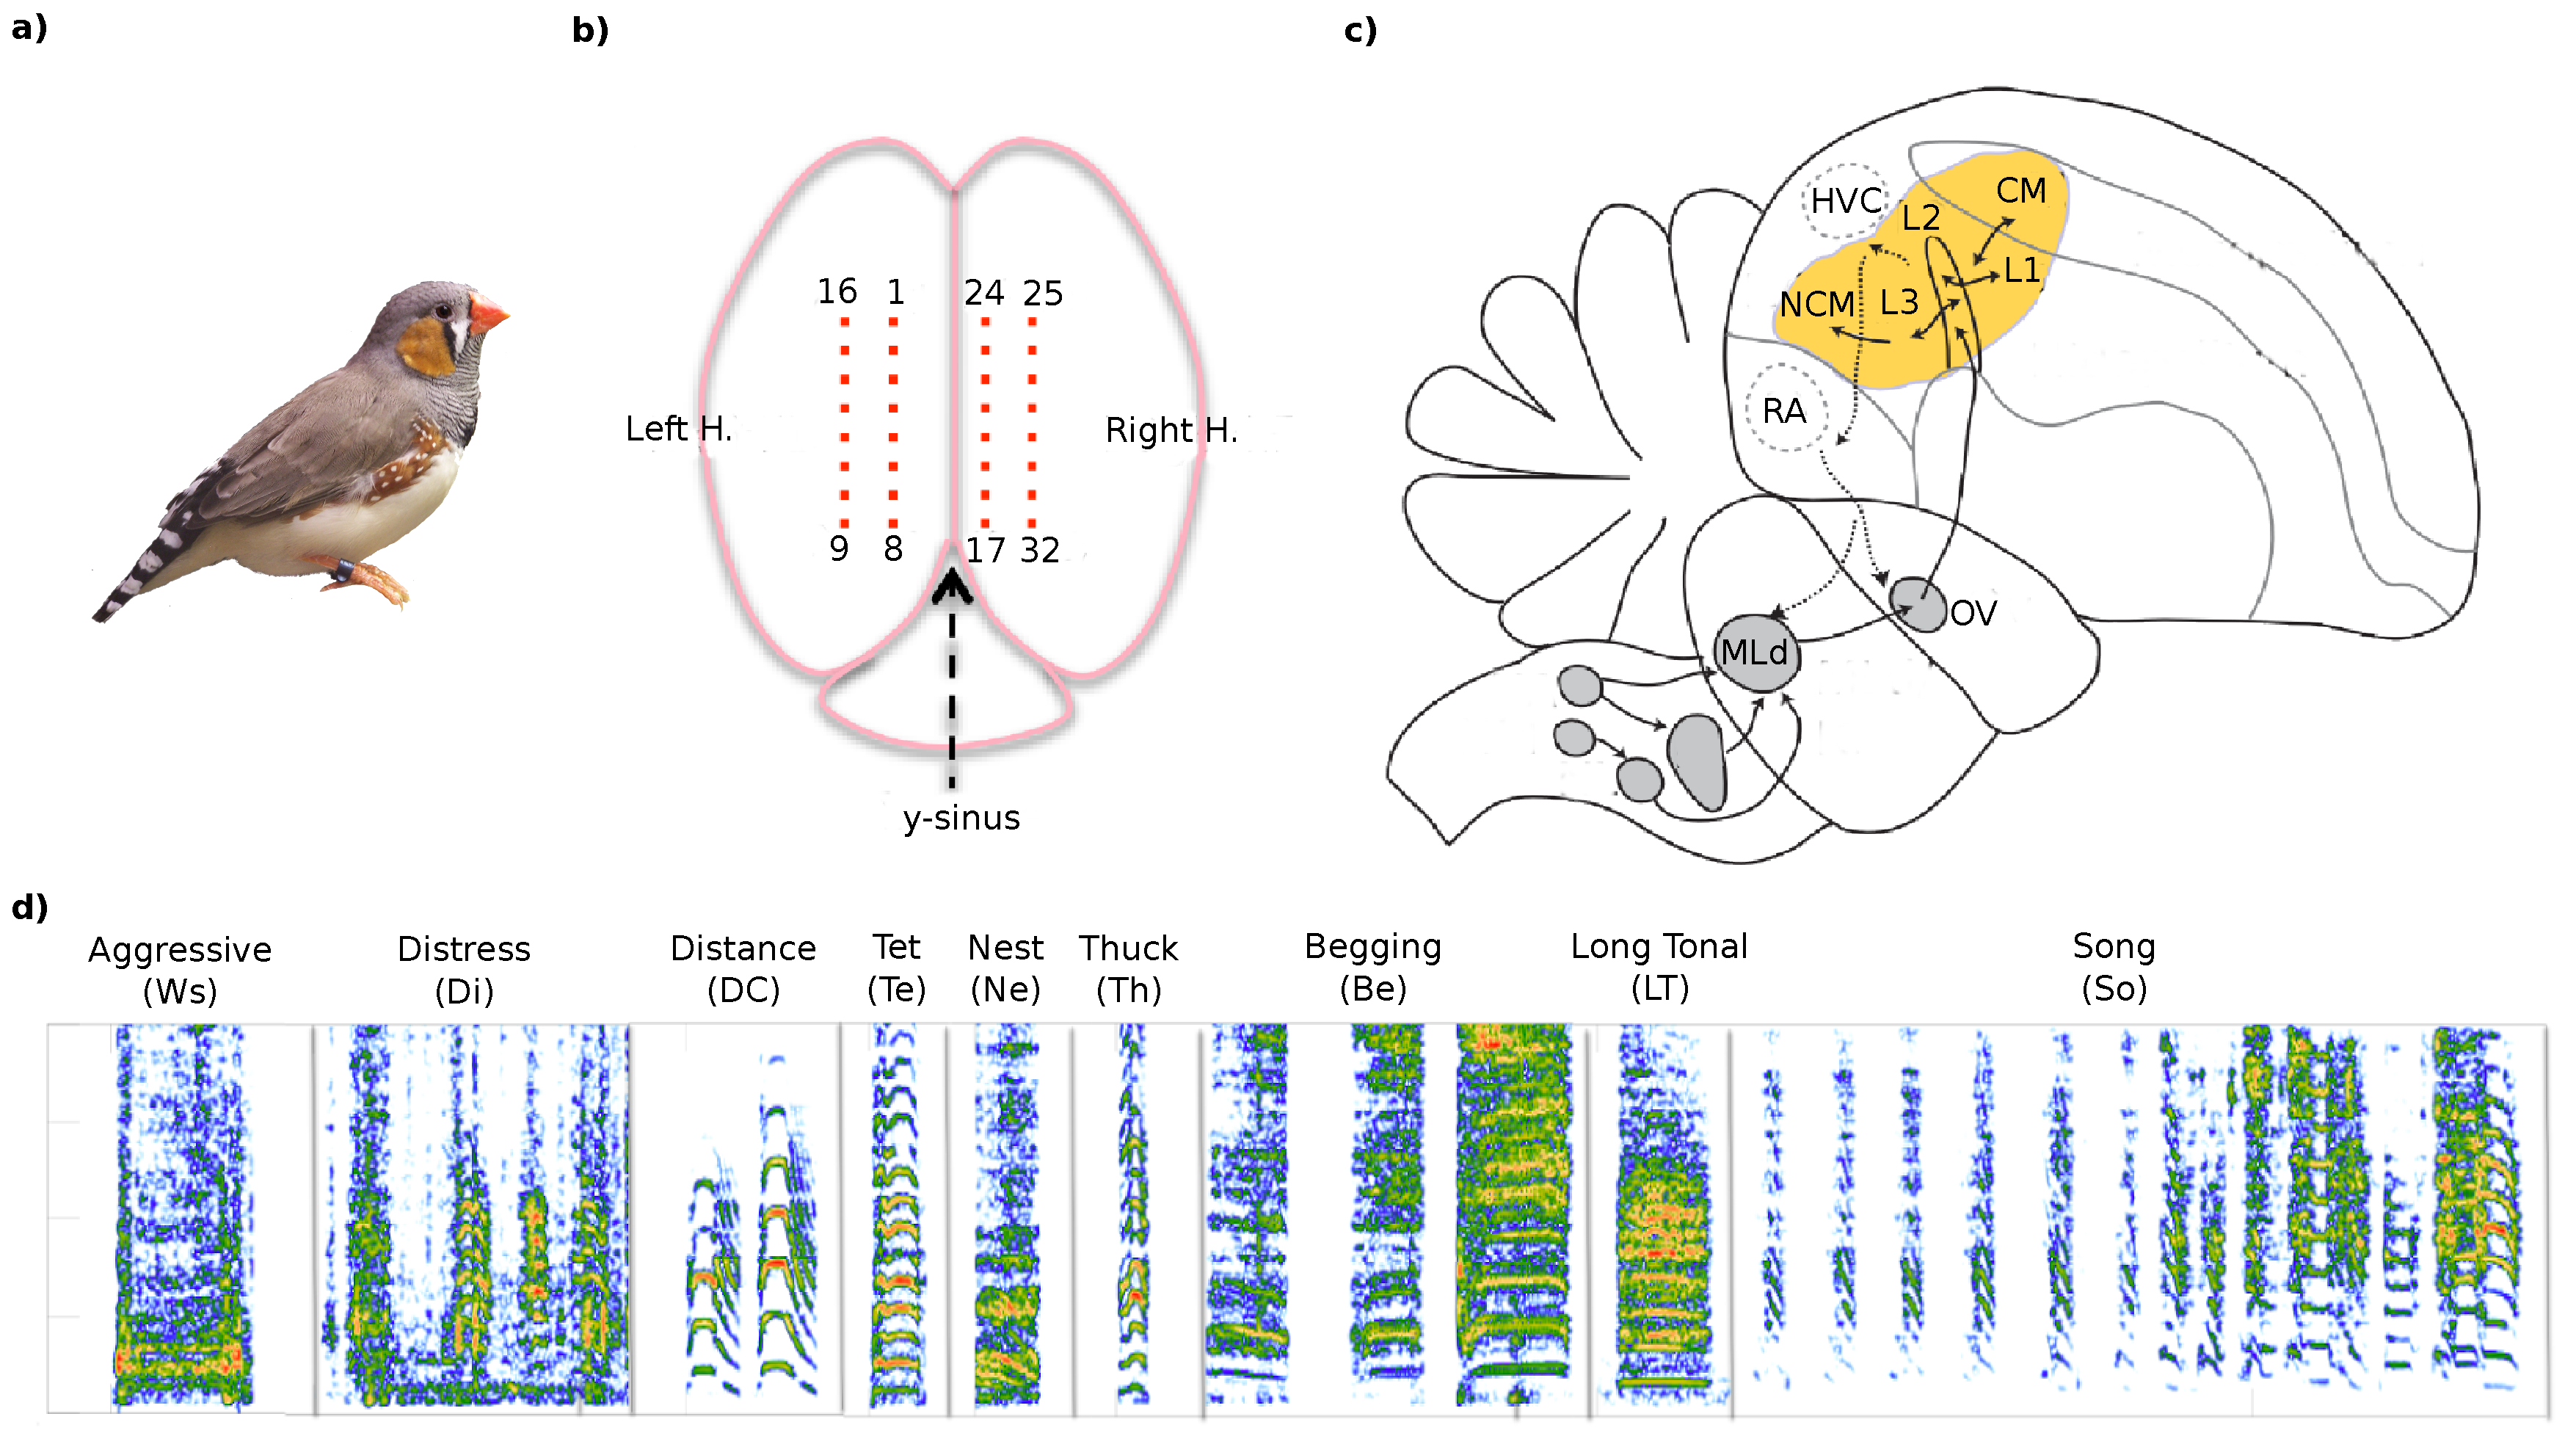
\includegraphics[scale=0.25]{figure1.eps}
\end{figure}

\subsection{Acoustic Features Covary and Cluster}

    Our goal is to describe how key features that characterize Zebra finch vocalizations are represented in neuronal spiking, and the LFP, as well as the relationship between neural spiking and the LFP. We segmented Zebra finch vocalizations and quantified their acoustic properties using a rich set of 20 acoustic features that characterized the syllable’s power spectrum, amplitude envelope, and the time-varying fundamental (see Methods - Acoustic Features). With the exception of temporal standard deviation ({\em Std T}), none of our features were dependent on the duration of syllables, that ranged in duration from 40ms to 400ms. {\em Std T} was linearly proportional to syllable duration (corrcoef=0.99). This produced a unique 20 dimensional feature vector for each syllable. It will be specifically noted when {\em Std T} is utilized in later analysis.

    In Figure 2, we show an example of the acoustic feature characterization for a single syllable, as well as examples of syllables that span the range of maximum amplitudes ({\em Max A}), mean spectral frequencies ({\em Mean S}) and pitch saliencies ({\em Saliency}). Saliency is a measure of syllable “pitchiness”, low for noisy syllables and high for harmonic-stack-like syllables. These features have been shown to be vital for determining the behavioral context, and hence semantic meaning, of Zebra finch vocalizations. Moreover, this set of features can be used in supervised classifiers to obtain identical discriminability performance of call types than the one obtained from a complete representation of the sound \cite{Elie2015b}.

\begin{figure}
    \caption{\textbf{Syllables quantified by acoustic features}: \textbf{(a)} an illustration of the acoustic features quantified for one syllable. The top plot shows the sound pressure waveform of a single syllable, with the amplitude envelope outlined in red. To the right in text are the temporal features quantified from the amplitude envelope and used in the study. The middle plot shows the power spectrum of the same syllable. Gray dotted lines indicate the first, second, and third quartiles of the spectral distribution ({\em Q1}, {\em Q2}, and {\em Q3}, respectively). {\em Q2} is the spectral median. Text to the right shows the values for the spectral features computed. The bottom plot of the left column shows a spectrogram of the syllable. The black dotted line indicates the mean fundamental frequency ({\em Mean F0}) computed from the time-varying fundamental. The text to the right shows the variety of features computed for the time-varying fundamental frequency. \textbf{(b)} Examples showing syllable variety along each acoustic feature axis. The top plot shows syllables ordered in increasing maximum amplitude, middle plot shows increasing mean spectral frequency, and bottom shows increasing saliency.}
    \centering
    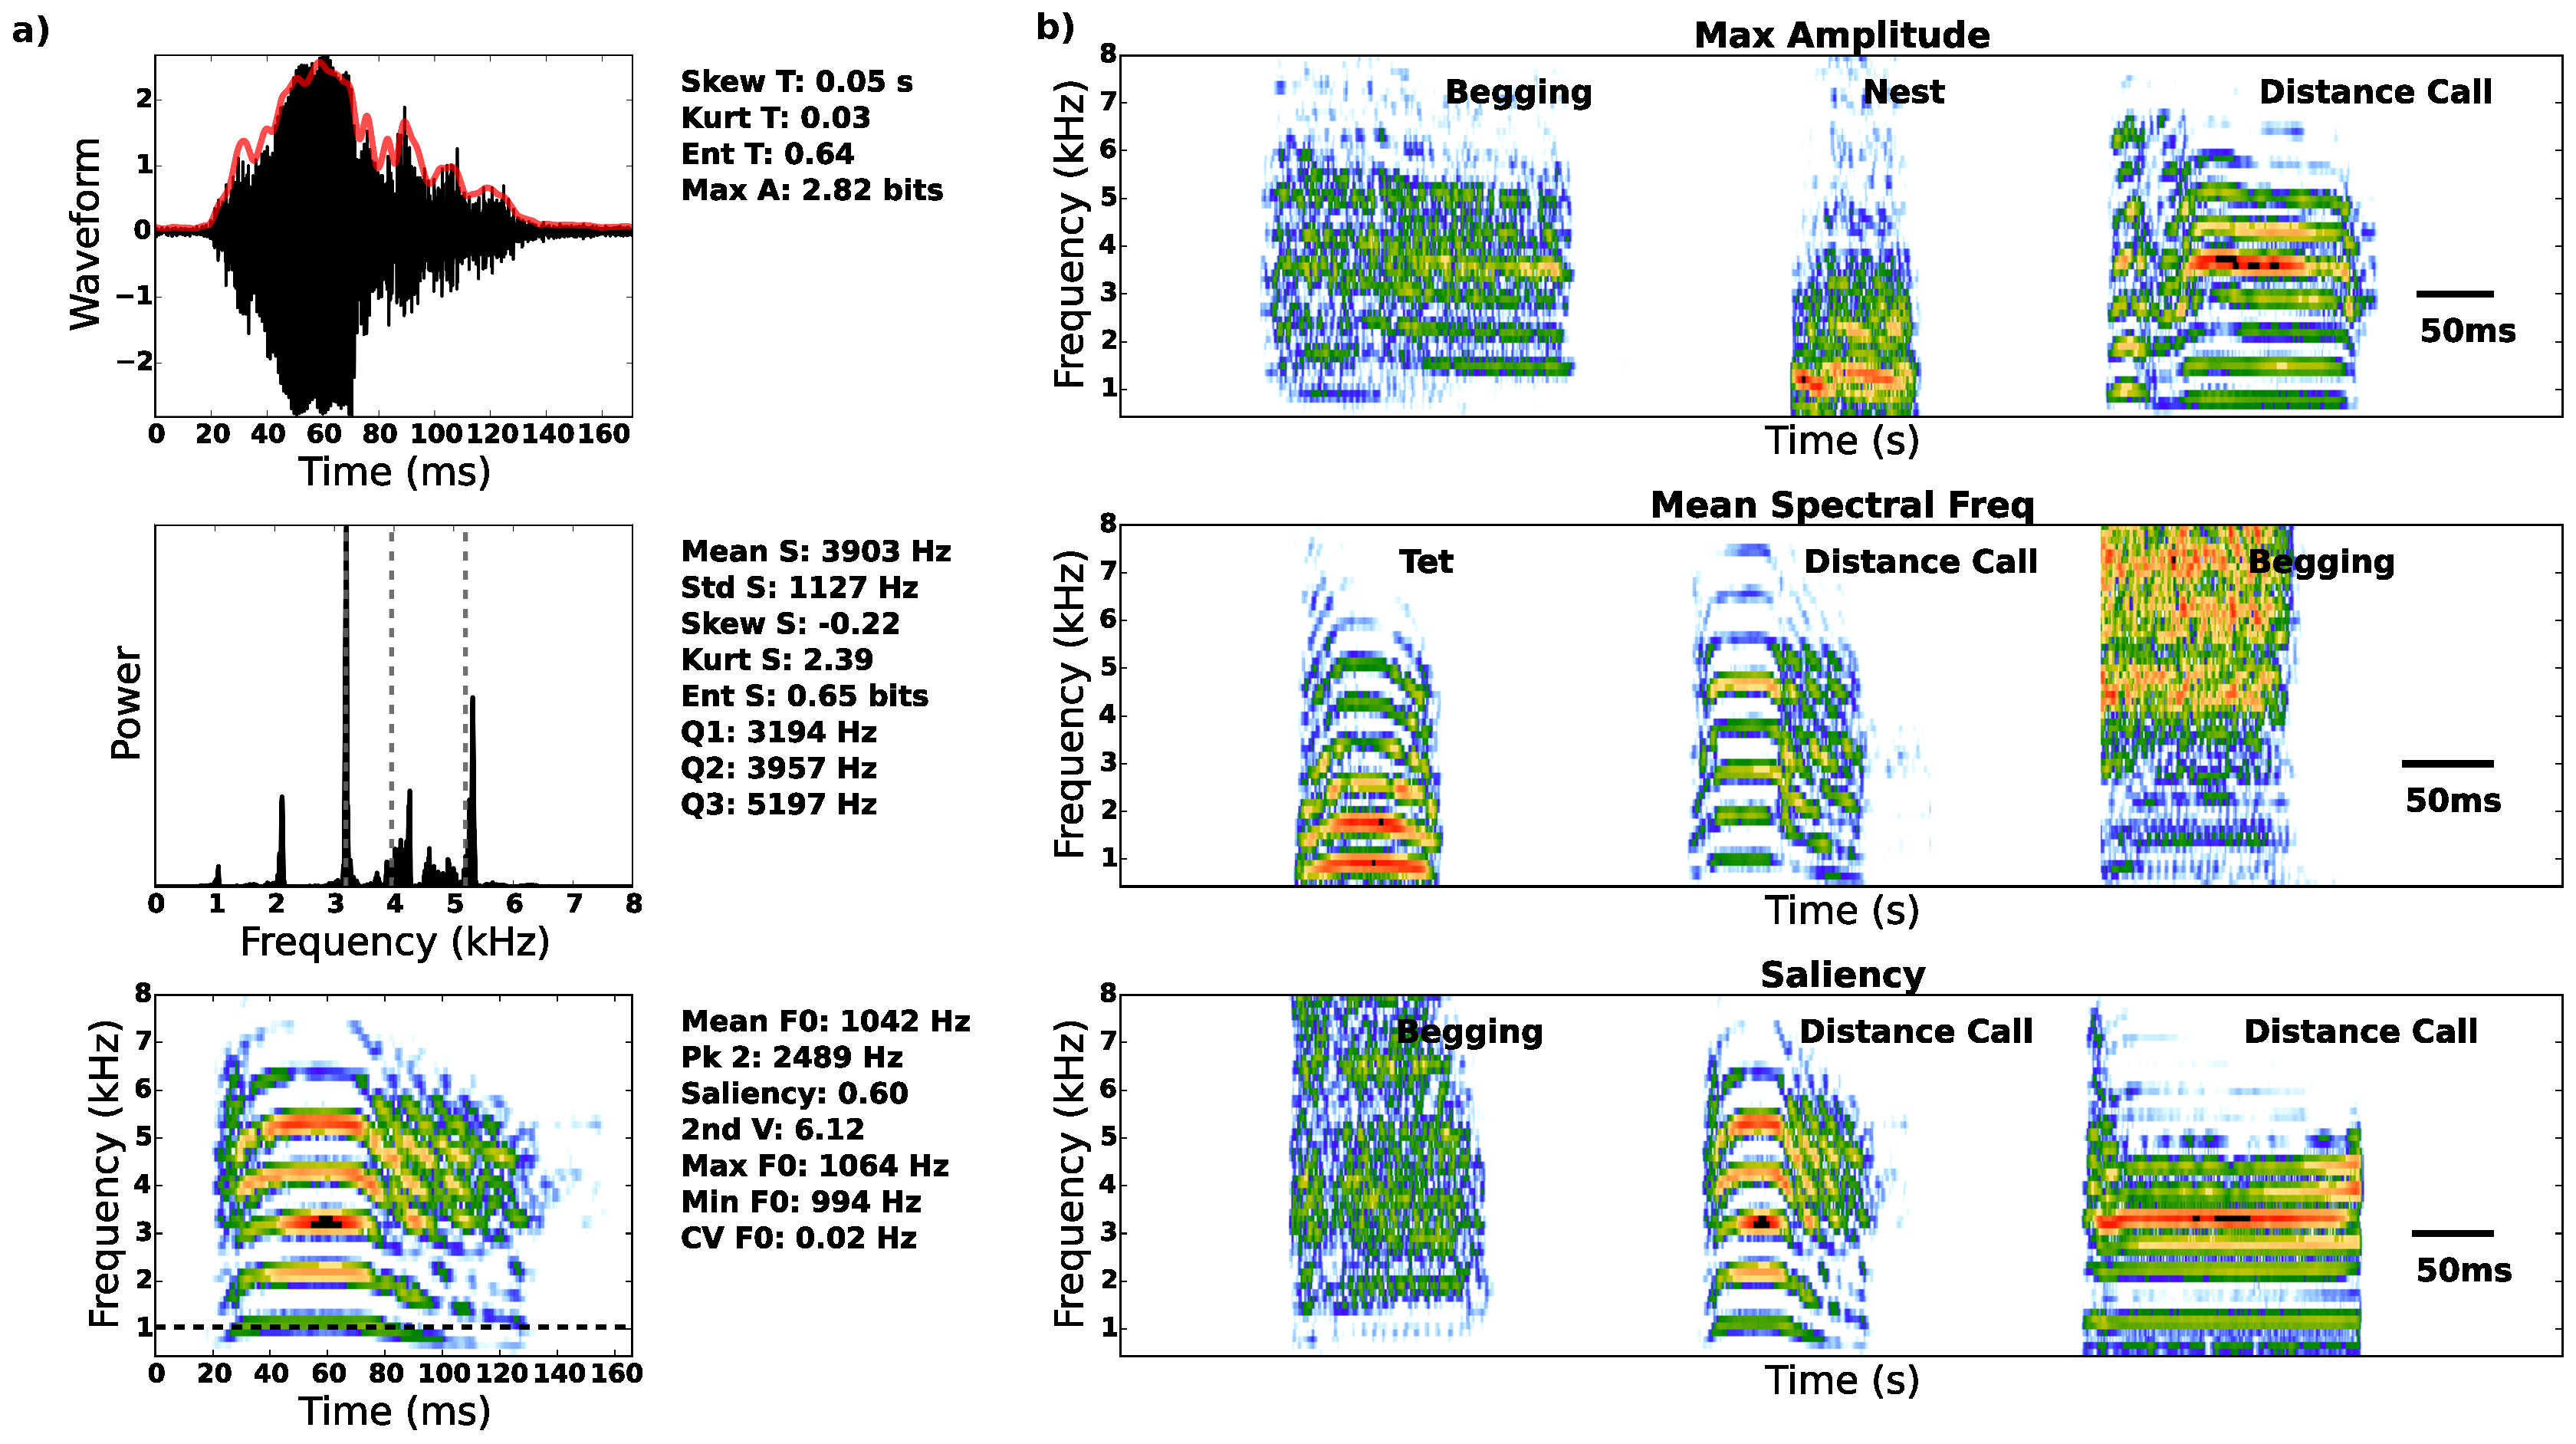
\includegraphics[scale=0.25]{figure2.eps}
\end{figure}

    Acoustic features are intuitive quantities for describing syllables, but are not completely independent of each other. By construction, they naturally fall into three groups - those that describe the spectral distribution, the temporal distribution, and the time-varying fundamental frequency. Figure 3a shows a matrix of correlation coefficients between each acoustic feature. The features are ordered according to constructed group, but also naturally fall into several groups given the block-diagonal structure of the correlation matrix. Figure 3b shows a manually organized graphical representation of acoustic feature relationships. Edge thickness depicts the absolute value of the correlation coefficient, and coefficients less than 0.20 are not shown.
Taken together, the correlation matrix and graph show that acoustic features cluster into several groups. The time-varying fundamental features form one group (green in Figure 3b), with the two parameters that describe the presence of a second voice ({\em Pk 2} and {\em 2nd V}) forming a distinct subgroup. Features that describe fundamental frequency over time, the mean ({\em Mean F0}), max ({\em Max F0}), min ({\em Min F0}), and coefficient of variation ({\em CV F0}) are strongly correlated with each other. Purely spectral features, statistics computed from the power spectrum of the syllable, form another group (orange in Figure 3b). The mean spectral frequency ({\em Mean S}), 25th, 50th, and 75th percentiles of the spectral distribution ({\em Q1}, {\em Q2}, {\em Q3}, respectively), and the spectral skew formed a strongly correlated subgroup. We note also that these spectral frequency parameters are only weakly correlated with the mean fundamental; in other words, birds can increase their fundamental frequencies while not changing the spectral envelope of the sound and vice-versa \cite{Elie2015b}. The spectral kurtosis ({\em Kurt S}) was correlated to spectral standard deviation ({\em Std S}). The spectral entropy {\em Ent S}, a measure of inharmonicity, was strongly negatively correlated with Saliency - harmonic stack like syllables have low spectral entropies and high saliency, while noisy syllables have high entropies and low saliency. Both saliency and spectral entropy were correlated with spectral standard deviation and kurtosis. Quantities that describe purely temporal features were computed from the amplitude envelope and formed the last group (blue in Figure 3b). The mean and standard deviation of the amplitude envelope (not shown), were linearly proportional to syllable duration. The entropy of the amplitude envelope, temporal entropy ({\em Ent T}), was strongly negatively correlated with maximum amplitude ({\em Max A}) - syllables with amplitude envelopes with high variation, such as Begging and Nest calls, also tended to have lower maximum amplitudes. Temporal skew ({\em Skew T}) and kurtosis ({\em Kurt T}) were correlated with each other but not much with other features.

\begin{figure}
    \caption{\textbf{Acoustic features cluster into groups}: \textbf{(a)} We performed a correlation analysis to show how the acoustic features were related to each other. The correlation matrix shows that the features fall into several clustered groups - spectrotemporal features involving fundamental frequency ({\em Mean F0} to {\em CV F0}), two clusters of spectral distribution features ({\em Std S} to {\em Ent S} and {\em Mean S} to {\em Skew S}), and temporal features ({\em Skew T} to {\em Max A}). \textbf{(b)} A graph of these features is shown, the width of the edge is proportional to the absolute value of the correlation coefficient between two features, and edges with magnitude less than 0.20 were discarded. The features are colored by their grouping (green = spectrotemporal, orange = spectral distribution, blue = temporal). Within-group edges are thicker than between-group edges. Not pictured, but utilized in the analysis, is the temporal standard deviation ({\em Std T}), which was linearly proportional to syllable duration, and uncorrelated to the other acoustic features.
}
    \centering
    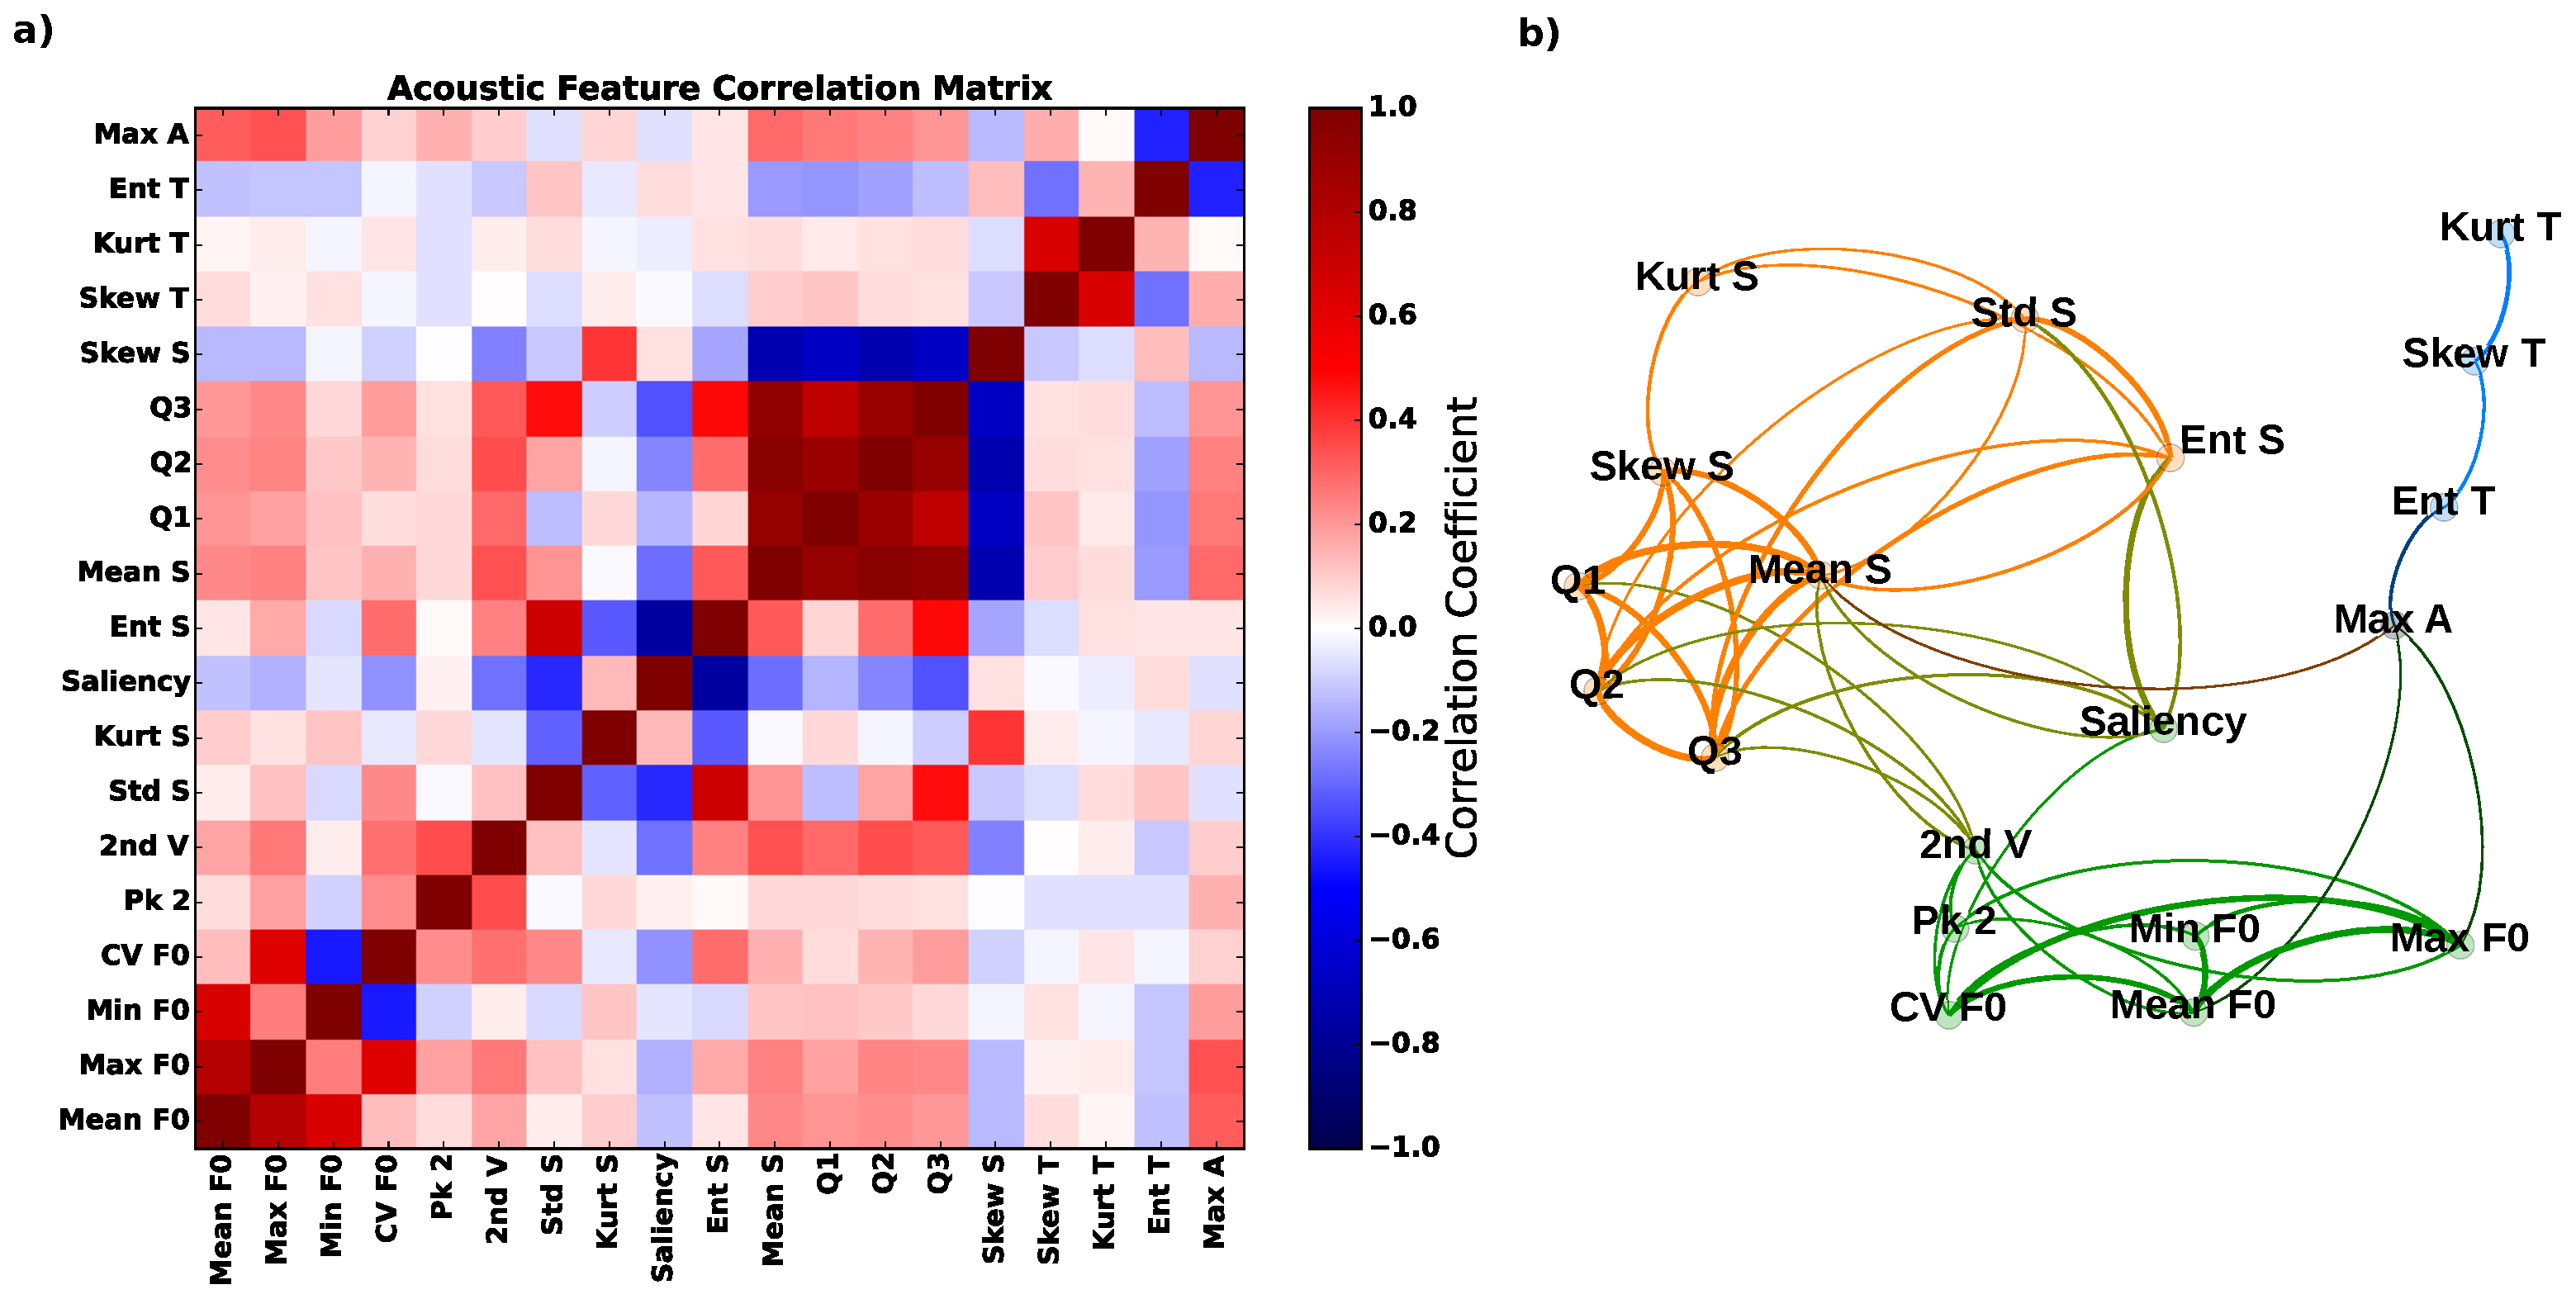
\includegraphics[scale=0.25]{figure3.eps}
\end{figure}


\subsection{How Spikes and LFP are Driven by Amplitude, Mean Spectral Frequency, Saliency}

    We used an encoder analysis to understand how acoustic features drive spike rate and LFP power. Figure 4 shows the isolation and extraction of features for syllables and the LFP. A syllable was isolated (Figure 4a), and the multi-electrode spike trains and LFP were taken for each of the ten trials the syllable was presented for (Figure 4c). The spike rate was computed for each trial, and averaged across trials. The power spectrum was computed from the LFP on each electrode for each trial, and the power spectra were averaged across trials to produce multi-electrode power spectra (Figure 4d). Performance of encoders and decoders for the LFP, described shortly, were contingent on first taking the log of the power spectra, and then z-scoring within electrode and frequency. The frequencies were then summed in three bins - 0-30Hz, 30-80Hz, and 80-190Hz.

\begin{figure}
    \caption{\textbf{Preprocessing of syllables and LFP}: An illustration of the methods used to transform the sound stimulus, multi-electrode local field potential, and spike trains. \textbf{(a)} A spectrogram of the vocalization, a male distance call (DC) which was emitted three times in a row. Dashed lines indicate the syllable chosen for visualization. The sequence of three call syllables was randomly repeated 10 times over the course of the recording session, along with other types of calls and songs that comprise the full vocal repertoire. \textbf{(b)} Acoustic features were computed for the syllable and z-scored across acoustic features for all syllables. The plot shows these properties for the selected syllable. \textbf{(c)} One trial of raw local field potential (LFP) recorded from a 8x2 multi-electrode array in the Zebra Finch auditory system, shown here for one trial. Electrodes are ordered rostral-caudal. \textbf{(d)} The z-scored multi-electrode LFP log power spectra, computed per trial and then averaged across trials. Each row corresponds to an electrode, and electrodes are ordered rostral-caudal, in the same order as (c). Frequency varies along the x-axis.
}
    \centering
    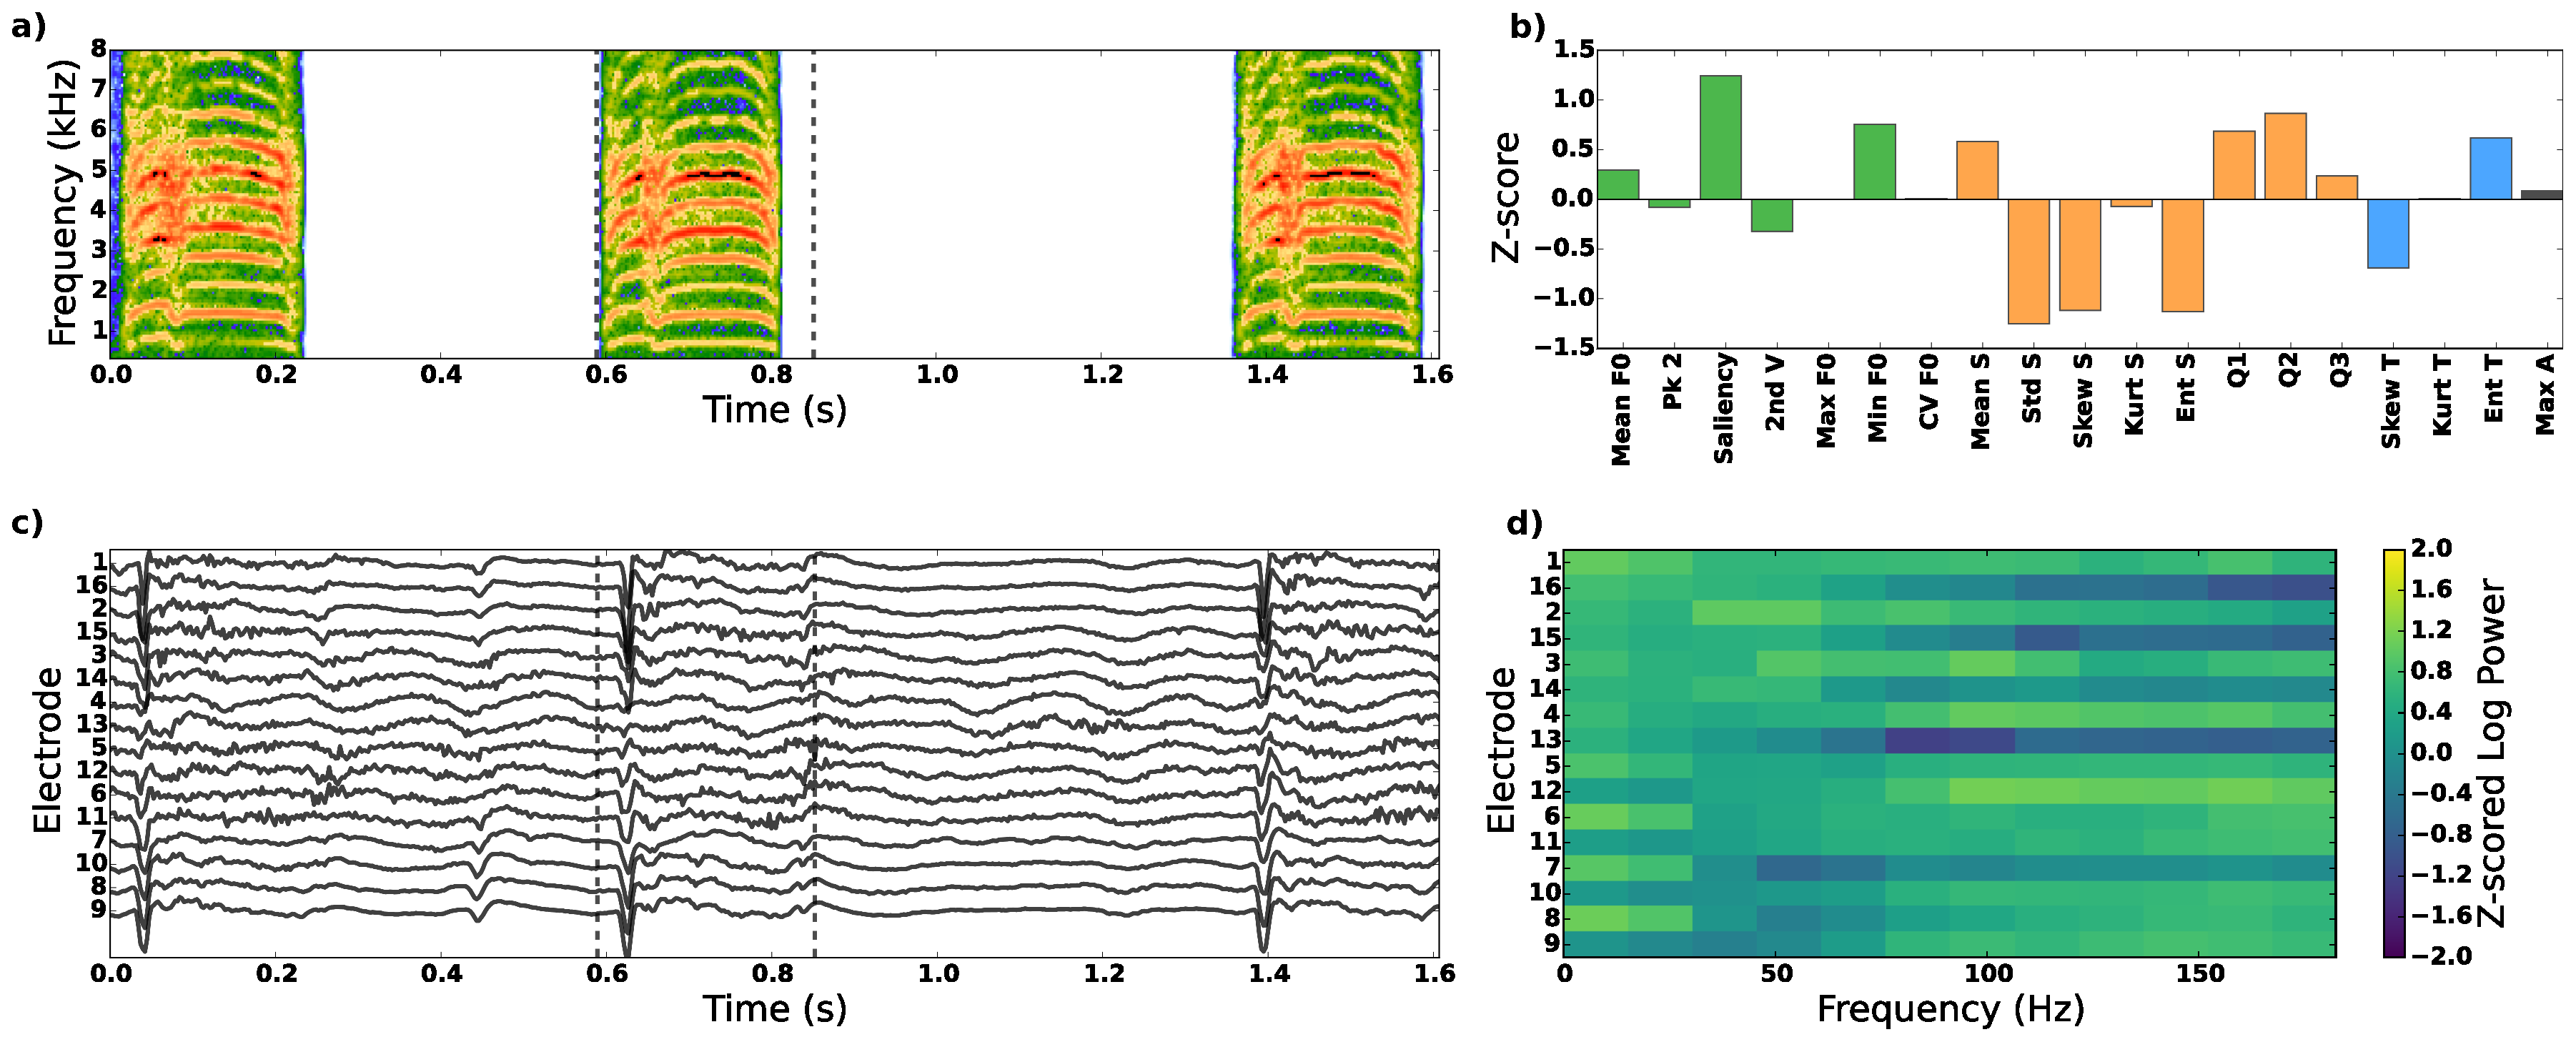
\includegraphics[scale=0.25]{figure4.eps}
\end{figure}

We used a stagewise procedure to build the encoder, meaning acoustic features were included in the encoder only if they boosted generalization performance, measured by the cross-validated R2 (see Methods - Encoder to Predict Spikes and LFP from Acoustic Features). However, because some of the acoustic features were highly correlated, we first chose a set of “baseline” features that were always included in the regression - maximum amplitude ({\em Max A}), mean spectral frequency ({\em Mean S}), and pitch saliency ({\em Saliency}). We used a nonlinear spline basis that allowed us to simultaneously fit nonlinear tuning curves between the neural response (spike rate or log power), and each acoustic feature (see Methods - Spline Basis Representation of Acoustic Features and Methods - Tuning Curves).

Figure 5a shows example tuning curves for several acoustic features, and the top row shows the curves for maximum amplitude ({\em Max A}). Strikingly, the neural response to amplitude is bimodal, some neurons respond to increases in amplitude by increasing their spike rate, while others decrease their spike rate (not shown). We quantified the tuning curves by computing their linear slope, ignoring slopes from models that had a cross-validated R2 of less than 0.05. Of the spike rate tuning curves for maximum amplitude (n=590), 62\% had negative slope (decreased with increasing amplitude). For 0-30Hz LFP (n=302), 85\% had a negative slope, while for 30-80Hz (n=396), 50\% of the tuning curves had negative slope, and for 80-190Hz (n=404), 47\% of the tuning curves had negative slope. No significant relationship was found between the anatomical corrdinates of a neuron or electrode, and the slope of the maximum amplitude tuning curve. Thus there are neurons that respond to increases in amplitude with increasing spike rate, and neurons that respond to increases in amplitude with a decreasing spike rate, and the same properties are reflected in tuning curves for the LFP.

The second row of Figure 5a illustrates that the relationship between spike rate or LFP power and mean spectral frequency is multimodal and nonlinear. Most spike rate tuning curves for mean spectral frequency had a negative slope (80\%, n=652), meaning spike rate decreased as mean spectral frequency increased. Some spike rate tuning curves had a local maximum peak (also called a “best frequency”) near 3kHz. Examining only the tuning curves that had an identifiable local maximum (not at the endpoints) in the 2-4kHz range, we found that 58\% (n=378) had an identifiable center frequency. The median center frequency of these tuning curves was 3.1kHz, with a standard deviation of 0.7kHz. The spike rate tuning curves were most similar to the 80-190Hz LFP band (Table 1). Tuning curves for 0-30Hz and 30-80Hz LFP were predominantly negative sloped, and had central peaks less often. No significant spatial relationship, i.e. tonotopy, was found between anatomical location and center frequency. To summarize, increases in mean spectral frequency most often decreased neural activity when measured by spike rate or LFP power. When tuning curves had a central peak, it was most often around 3kHz.

\begin{table}
\begin{center}
\begin{tabular}{|p{2.4cm}|p{2.4cm}|p{2.4cm}|p{2.4cm}|p{2.4cm}|p{2.2cm} |}
\hline
 & \textbf{N} & \textbf{\% Negative Slope} &
\textbf{\# Central Peaked Tuning Curves} & \textbf{Median Center Frequency (Hz)} &
\textbf{Center Frequency SD} \\
\hline 
\textbf{Spike Rate} & 652 & 79\% & 378 & 3155 & 746 \\
\hline 
\textbf{LFP Power (0-30Hz)} & 310 & 96\% & 68 & 3236 & 1082 \\
\hline 
\textbf{LFP Power (30-80Hz)} & 425 & 96\% & 138 & 3351 & 1147 \\
\hline 
\textbf{LFP Power (80-190Hz)} & 421 & 78\% & 193 & 3351 & 886\\
\hline
\end{tabular}
\end{center}
\caption{Tuning Curve Statistics for Mean Spectral Frequency}
\end{table}

In the third row of Figure 5a we show example tuning curves for saliency. The curves exhibit some bimodality (positive and negative slopes). For spike rate tuning curves (n=620), 44\% had a negative slope, while for 0-30Hz LFP (n=301) and 30-80Hz LFP (n=344), only 20\%  and 30\% of the tuning curves had negative slopes, respectively.  For the 80-190Hz frequency band, 40\% (n=355) of the tuning curves had a negative slope, similar to spike rate tuning curves. The tuning curves for temporal skew (Skew T) overwhelmingly exhibited negative slopes, the percentage of negative-sloped tuning curves was greater than 95\% for spike rate, and all LFP frequency bands.

\begin{figure}
    \caption{\textbf{How spikes and LFP power are driven by amplitude, spectral mean, saliency}: We built encoders to predict spikes or LFP power from nonlinearly mapped acoustic features. The encoder fit tuning curves simultaneously across acoustic features, and a weighted combination of tuning curve outputs were used to predict neural activity. \textbf{(a)} Tuning curves across sites for a subset of neurons, relating spike rate to acoustic features (first column). The subsequent columns show the mapping between LFP power in three different frequency bands (0-30Hz, second column, 30-80Hz third column, 80-190Hz fourth column). Tuning curves are shown for maximum amplitude ({\em Max A}, first row), mean spectral frequency ({\em Mean S}, second row), saliency (third row), and temporal skew ({\em Skew T}, fourth row). \textbf{(b)}  In addition to the baseline features {\em Max A}, {\em Mean S}, and {\em Saliency}, other acoustic features were included using a stagewise regression if they improved encoder performance above baseline. The plot shows the fraction of times an acoustic feature was included in the regression, when predicting spike rate (first column), or one of the LFP power frequency bands (next three columns). \textbf{(c)} A boxplot of encoder performance for neurons (first box, red) and LFP power by frequency bands (subsequent columns, blue).
}
    \centering
    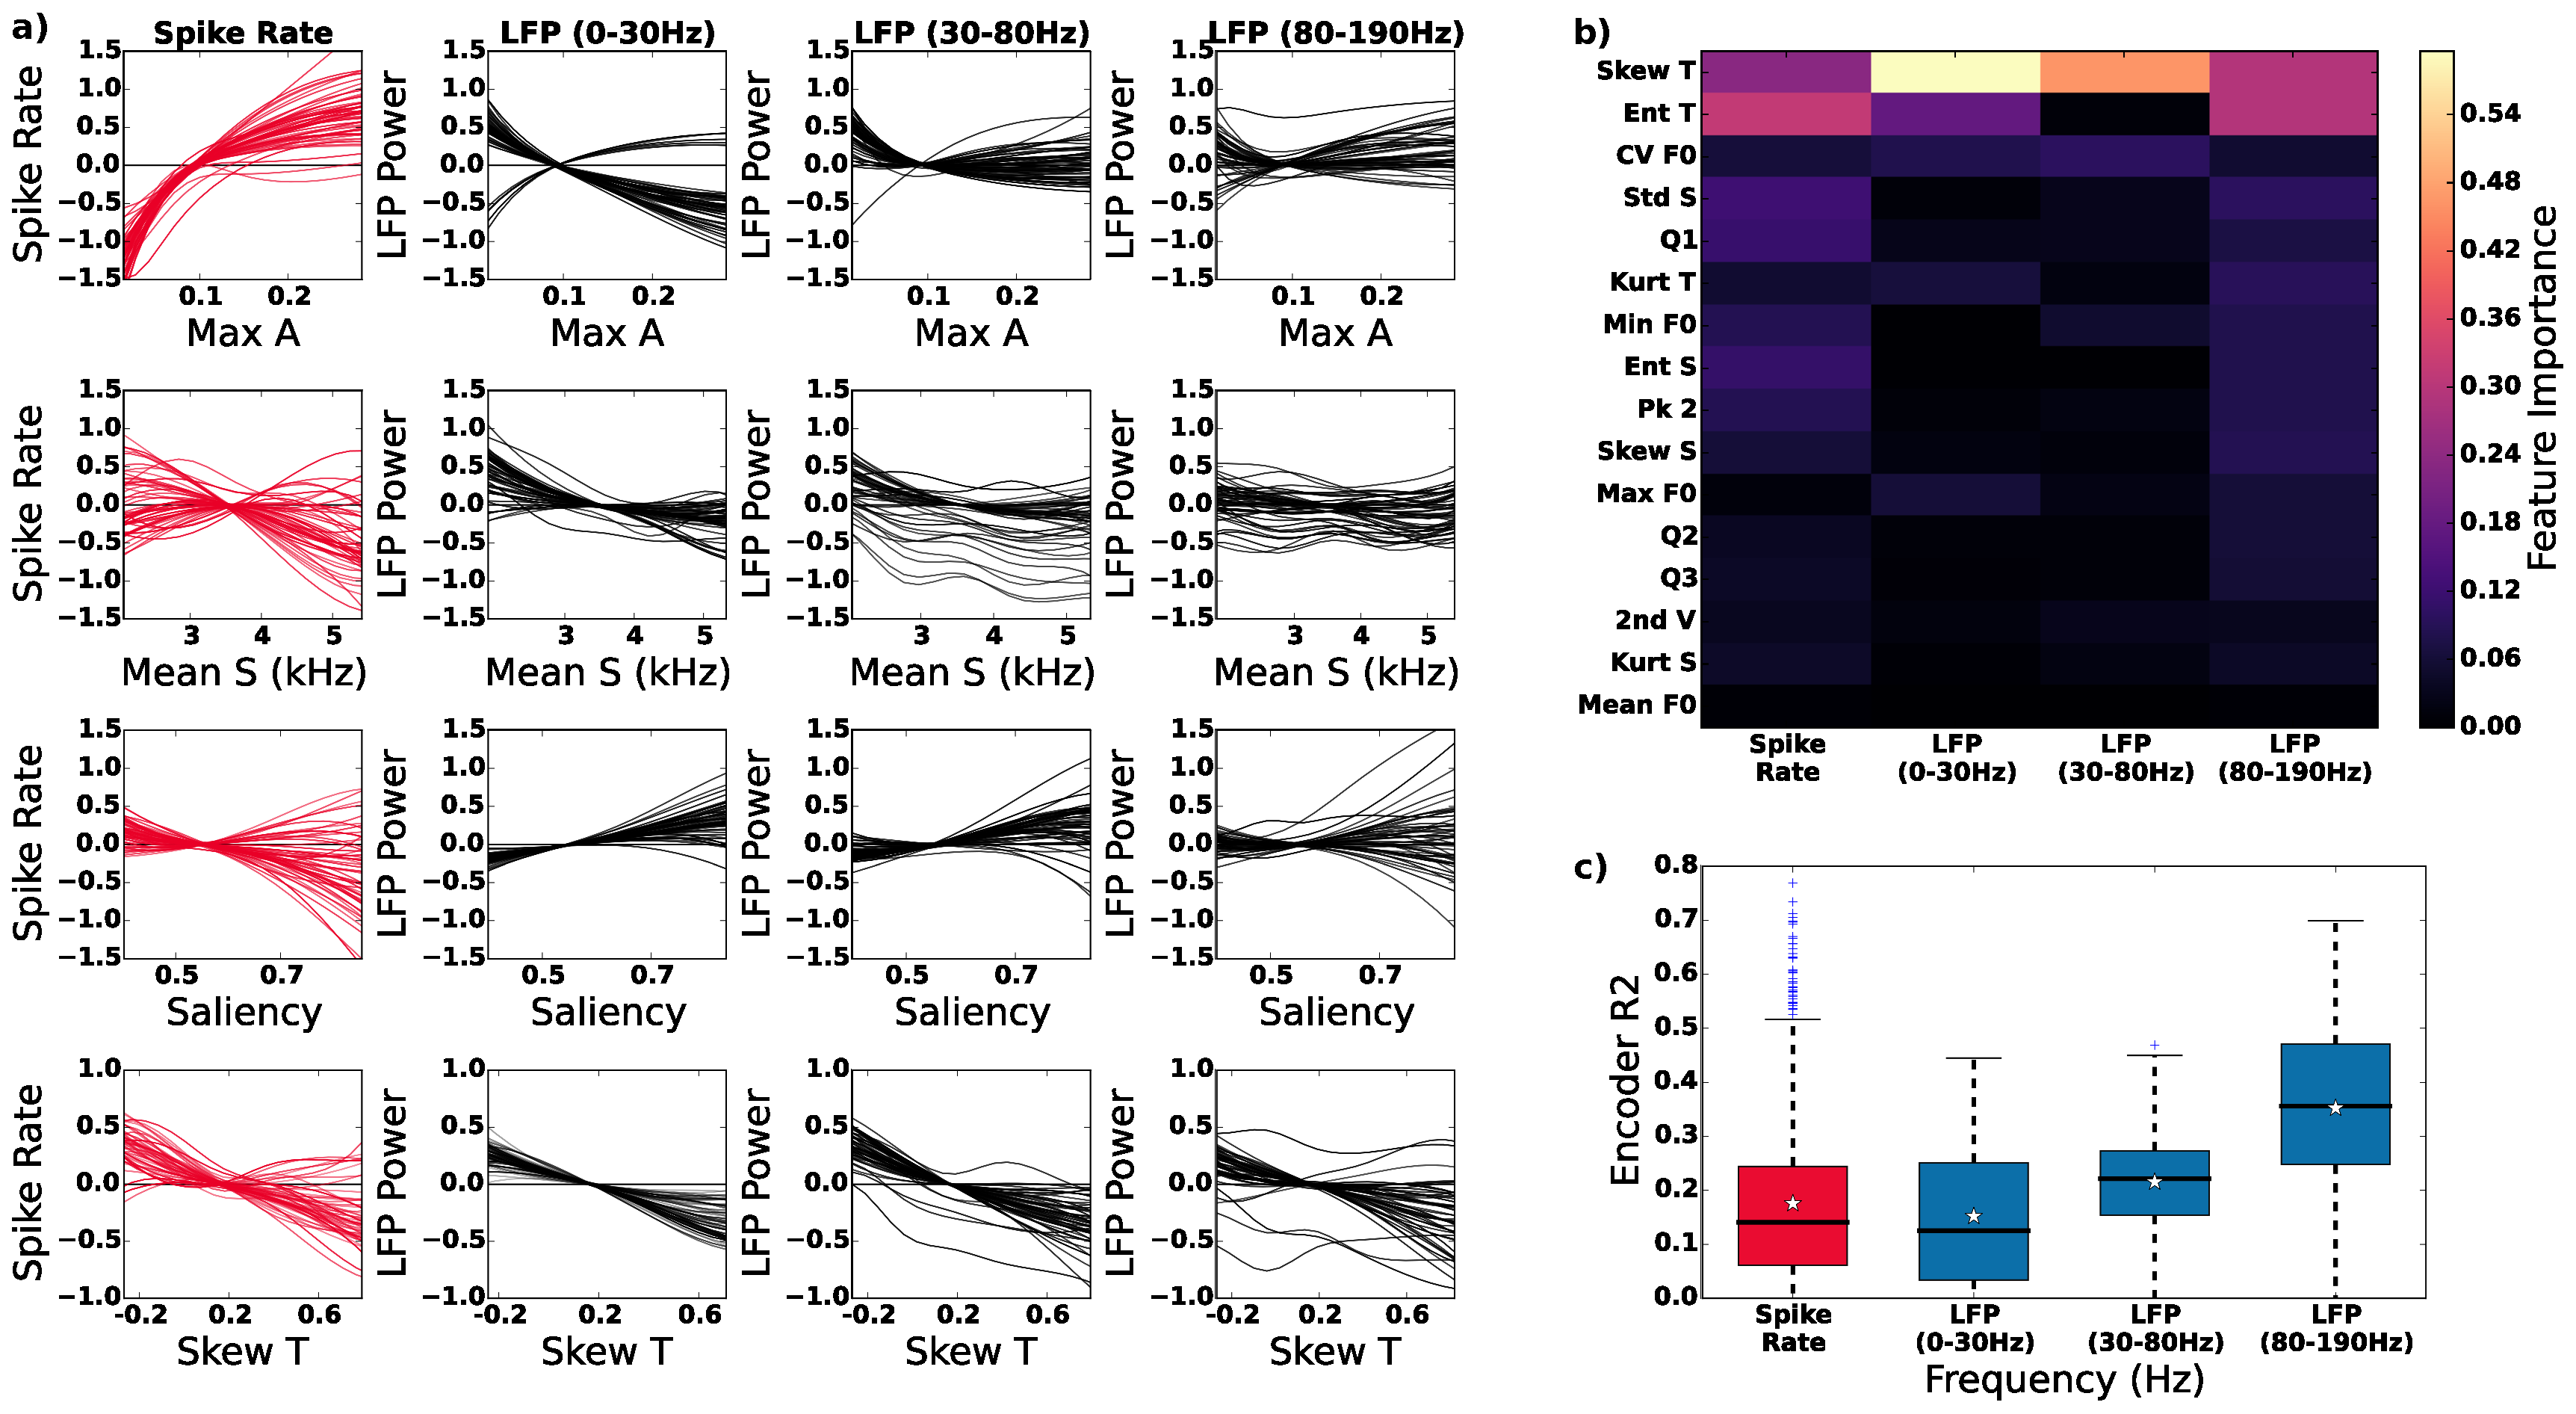
\includegraphics[scale=0.25]{figure5.eps}
\end{figure}

The stagewise approach we utilized to fit our encoder allowed us to determine how important non-baseline acoustic features were in predicting neural activity. Figure 5b shows the fraction of times that a non-baseline acoustic feature was included in the analysis (``Feature Importance''). It is important to note that we allowed temporal standard deviation ({\em Std T}) to be a feature. {\em Std T} is linearly proportional to syllable duration, and was included in a significant fraction ($>$ 90\%) of encoders for the 0-30Hz and 30-80Hz frequency bands, though it is not displayed in Figure 5b. The temporal skew ({\em Skew T}) and temporal entropy ({\em Ent T}) were the top non-baseline features utilized by the encoders, with the rest of the acoustic features being rarely included.

    The overall performance for the encoders, quantified by the cross-validated R2, is shown in Figure 5c for all LFP frequency bands spike rate. There was a significant effect of neural signal representation on encoder performance (ANOVA, F(3, 1631)=164, p$<$0.01), with the encoder models performing best for high frequency LFP (80-190Hz). There was also a significant, albeit smaller effect of region on encoder performance (ANOVA, F(5, 1629)=9, p$<$0.01); the encoders performed best for neurons/electrodes in region CM, and worst for region NCM. To summarize the results in this section, we successfully predicted spike rates for most neurons, and LFP power for most electrodes, with our encoder models. Neural responses were found to covary with amplitude (Max A) and saliency ({\em Saliency}) in a bimodal fashion, with some neurons/electrodes decreasing their response to increases in those variables, and others decreasing their response. Neural activity typically decreased with increasing mean spectral frequency ({\em Mean S}) or temporal skew ({\em Skew T}).

\subsection{Regional Specificity in Single Electrode Decoding Performance}

We built decoders to predict individual acoustic features from multi-band LFP power on individual electrodes to investigate whether there is regional specificity in decoding performance, before exploring ensemble decoding. The panels in Figure 6a show single electrode decoder performance across space, for all electrodes across recording sites, with electrodes from the two hemispheres plotted together as a function of their distance from the midline along the medial-lateral axis, and their rostral-caudal distance from region L2A. Figure 6b shows the regions that correspond to the plotted electrode locations. Figure 6c shows single electrode decoder performance (cross-validated R2) averaged within acoustic feature and anatomical region. Regional specificity in decoding performance was tested for the representative features shown in Figure 6a. Maximum amplitude ({\em Max A}) was best decoded from regions L2 and L1 (ANOVA, F(4, 302)=9.1, p$<$0.01), while mean spectral frequency ({\em Mean S}) was best decoded from regions L2 and L3 (ANOVA, F(4, 309)=9.1, p$<$0.01). Saliency had less regional specificity, but was best decoded from region CM (ANOVA, F(4, 311)=7.5, p$<$0.01). Temporal skew ({\em Skew T}) had very little regional specificity, but was best decoded from L3 (ANOVA, F(4, 286)=3.2, p=0.01). These results show that amplitude and frequency can be best decoded from electrodes in regions CM and L1, L2, L3. 

\begin{figure}
    \caption{\textbf{Regional specificity of single electrode decoder performance}: Decoders were trained to predict acoustic feature values from the full LFP power spectrum of single electrodes. \textbf{(a)} Maps of single electrode decoder performance by anatomical location. Electrodes on left and right hemisphere are plotted together, with the left hemisphere points mirrored to correspond to the right hemisphere anatomical coordinates. \textbf{(b)} The anatomical region that corresponds to each electrode. \textbf{(c)} The R2 across electrodes, averaged within acoustic property and region.
}
    \centering
    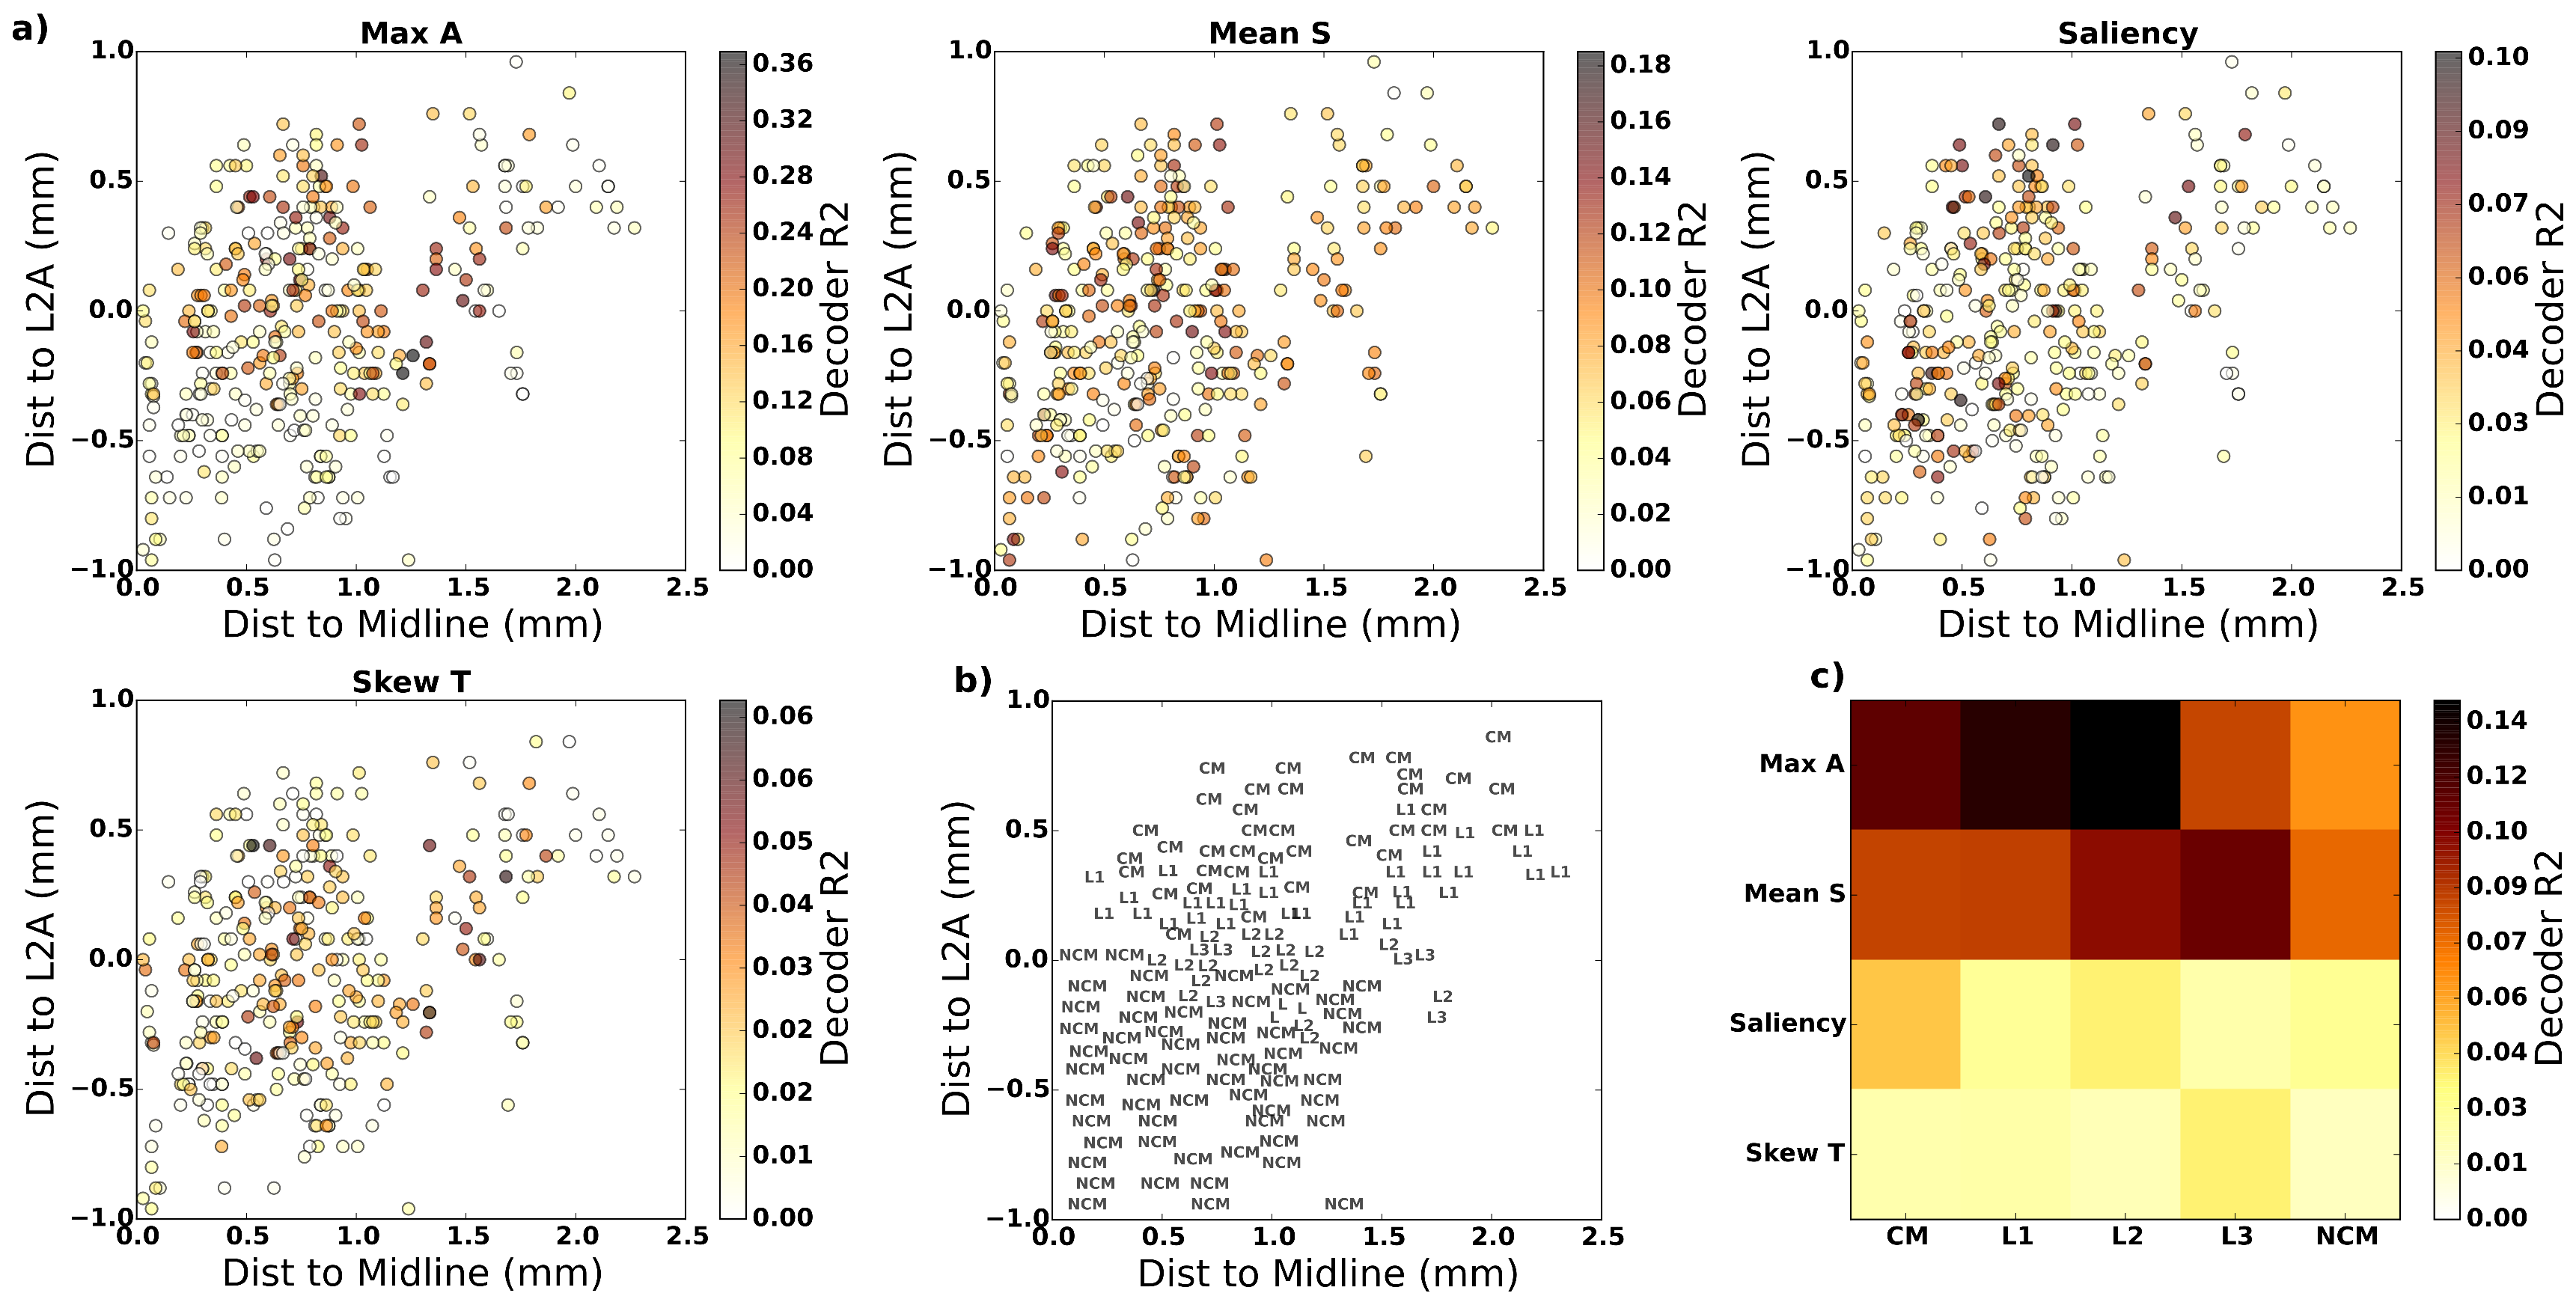
\includegraphics[scale=0.25]{figure6.eps}
\end{figure}


\subsection{Acoustic Features Decoded from Ensemble Activity}

Our encoder analysis demonstrated that neuronal spike rates and LFP power are driven by maximum amplitude ({\em Max A}), mean spectral frequency ({\em Mean S}), pitch saliency ({\em Saliency}), and temporal skew ({\em Skew T}), and our single electrode decoding analysis showed that these features can be decoded, with some regional specificity. Training decoders to predict individual acoustic features from ensemble activity allows us to explore how much information is contained in the population code and whether pairwise correlations improve decoder performance. So we built ensemble decoders to predict each individual acoustic feature from ensemble activity, represented by the population spike rate vector, LFP power spectra, or pairwise spike synchrony (Methods - Encoder and Decoder Dataset Construction). We utilized a simple measure of zero-lag pairwise synchrony, equal to the normalized dot product between two binary spike trains, and included synchrony terms for all pairs of neurons in an ensemble as input features to the decoder.

Figure 7a shows the mean performance by neural response type and acoustic feature. First, we found that including pairwise spike synchrony improved decoder performance for maximum amplitude ({\em Max A}) and spectral shape features ({\em Mean S}, {\em Q2}, {\em Q3}, {\em Skew S}, paired t-test, p$<$0.01 for all comparisons). No significant difference in performance was found between the population spike rate vector and multi-electrode LFP power spectra for those features (paired t-test, p$>$0.01 for all comparisons). Saliency and spectral entropy ({\em Ent S}) were best encoded by spike rate, which outperformed the multi-electrode LFP power spectra. LFP spectra outperformed spike rate and synchrony for temporal entropy ({\em Ent T}) and temporal skew ({\em Skew T}), implying that the power spectra representation contains more information about temporal properties than spike rate. To summarize, syllable amplitude and spectral shape are best decoded from population activity, and pairwise synchrony terms contain information about acoustic features that is not captured by the population spike rate vector.

\begin{table}
\begin{center}
\begin{tabular}{|p{2.4cm}|p{2.4cm}|p{2.4cm}|p{2.4cm}|p{2.4cm}|p{2.2cm} |}
\hline
 & \textbf{\em Max A} & \textbf{\em Mean S} &
\textbf{\em Saliency} & \textbf{\em Skew S} &
\textbf{\em Skew T} \\
\hline 
\textbf{Pop. Spike Rate} & 30 +/- 2 & 24 +/- 1 & 34 +/- 3 & 28 +/- 2 & 24 +/- 3 \\
\hline 
\textbf{Multi-electrode LFP} & 18 +/- 1 & 15 +/- 1 & 20 +/- 1 & 21 +/- 1 & 21 +/- 2 \\
\hline
\end{tabular}
\end{center}
\caption{ Average number of neurons electrodes needed to decode acoustic features to 90\% of peak ensemble decoding performance. Average was taken over dual-hemisphere recording sites, numbers listed are mean +/- stderr.}
\end{table}

We further investigated how decoder performance increased as a function of number of electrodes. To do this, we first merged electrodes from each hemisphere for each recording site, providing up to 32 electrodes which we utilized to decode individual acoustic features. Through spike sorting we obtained 1-3 cells per electrode, and utilized up to 60 neurons. For the population spike rate vector and multi-electrode LFP spectra, we ran a decoder for a variety of combinations of electrodes for a fixed number of electrodes (Methods - Ensemble Decoding Analysis). The results are shown in Figure 7b and 7c. Each curve within a plot shows the average cross-validation R2 for a fixed number of electrodes/neurons, from a dual-hemisphere recording site. We quantified the number of neurons necessary to reach 90\% peak decoder performance, across recording sites. We found that, when decoding from population spike rate, 25-30 neurons were needed to reach the 90\% peak decoder performance, while decoding from LFP power spectra, 15-20 electrodes were required (Table 2). Given that ensemble decoding performance greatly outperforms single electrode performance, we conclude that the neural representation of these key acoustical features in the avian auditory system is based on a distributed ensemble code. Also, given that only up to half of the number of electrodes/neurons were needed to reach near-peak performance, we conclude that there is redundancy in that code.

\begin{figure}
    \caption{\textbf{Ensemble decoding boosts performance}: \textbf{(a)} Decoders were trained on individual electrode arrays from each hemisphere (16 electrodes) to predict each acoustic feature, from the population spike rate vector (red), LFP power spectra (blue), and pairwise spike synchrony (brown). Adding pairwise synchrony terms to population spike rate vector typically boosted neuron decoding performance to that of spikes and LFP power. \textbf{(b)} Average spike rate decoder performance was estimated as a function of the number of neurons from combined dual-hemisphere recordings. \textbf{(c)} Average LFP PSD decoder performance was estimated as a function of number of electrodes for combined dual-hemisphere recordings (32 electrodes total) at each site.
}
    \centering
    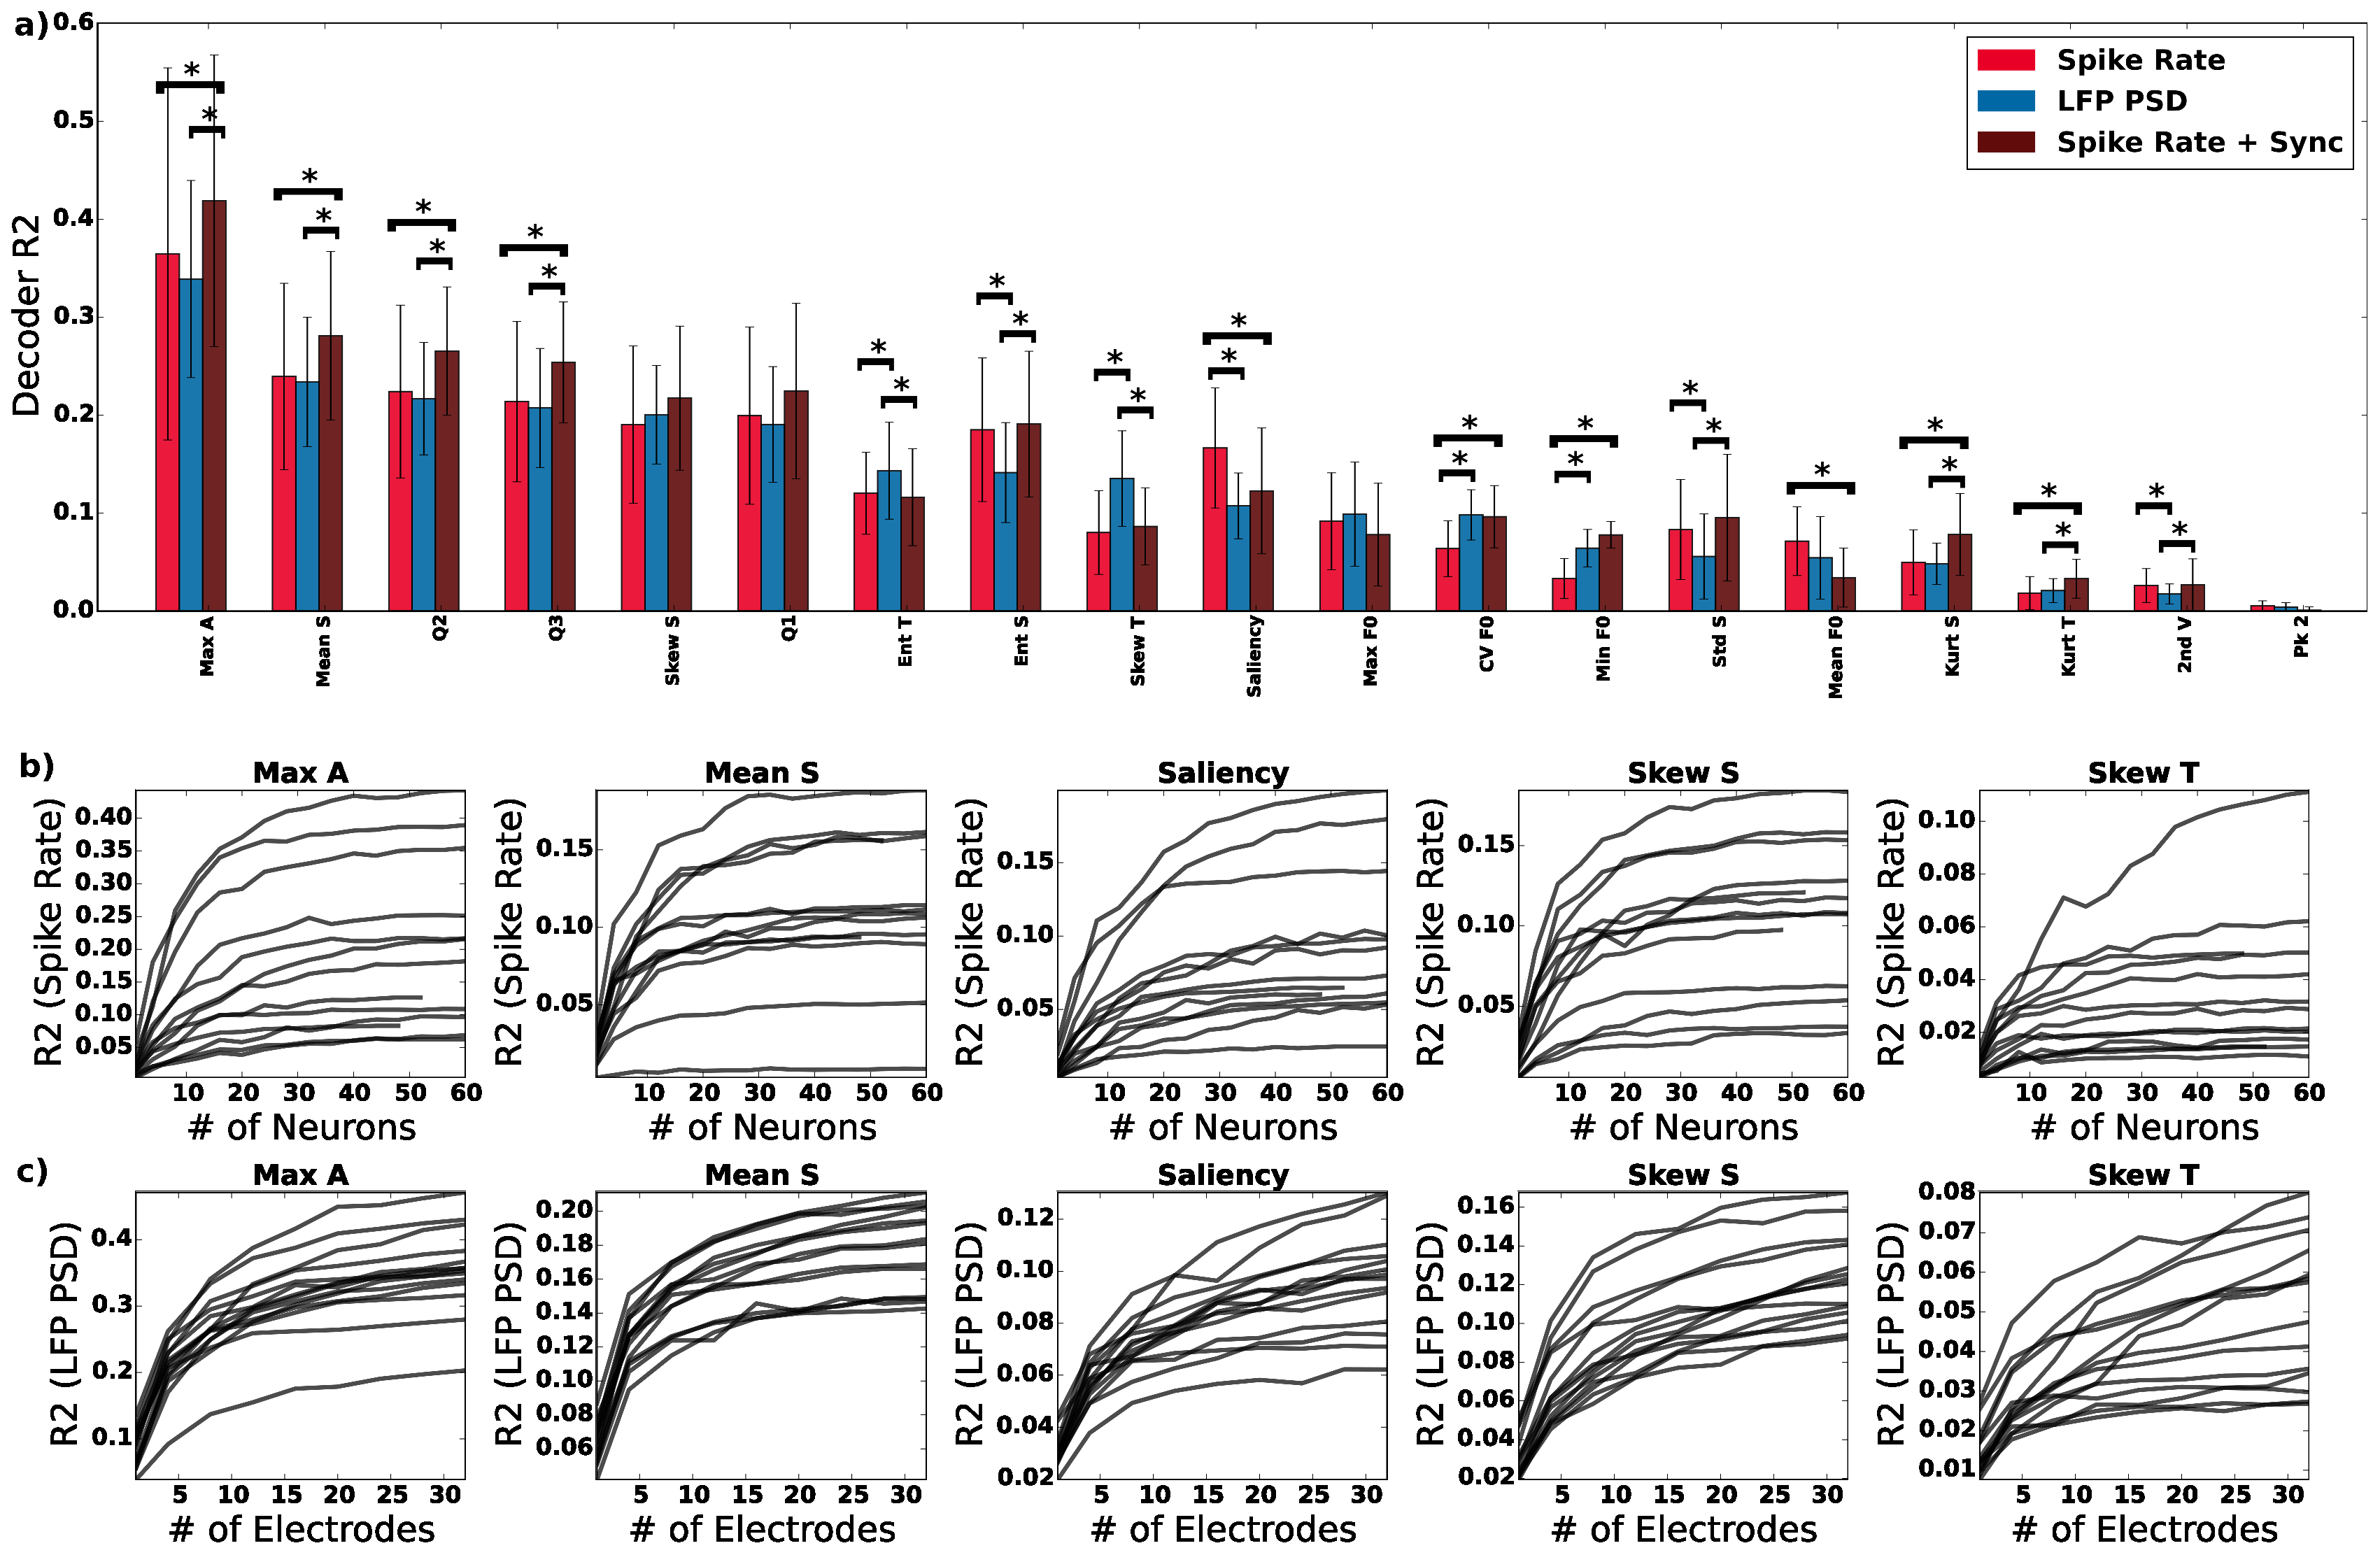
\includegraphics[scale=0.25]{figure7.eps}
\end{figure}

\subsection{LFP Power is a Mix of Local Population Spike Rate and Synchrony}

    The relationship between population spike activity and LFP power has not been directly quantified, so we built encoder models to predict LFP power in a given frequency band directly from population spike rate. In addition, we explored if spike synchrony better predicted LFP power (see Methods - Population Spike Rate and Spike Synchrony and Methods - Spike Rate to LFP Power Encoder). Figure 8a shows that LFP power can be predicted robustly by population spike rate. Adding spike synchrony terms improves predictive performance for the 30-80Hz and 80-190Hz bands (paired t-test, p$<$0.01 for all comparisons). For spike rate alone, performance increased with increasing frequency (ANOVA, F(2, 875)=62.5, p$<$0.01). The same was true for spike rate combined with spike synchrony (ANOVA, F(2, 880)=281.8, p$<$0.01). To summarize, the results in Figure 8a demonstrate that the LFP can be predicted best at high frequencies, by a combination of population spike rate and spike synchrony. 

The LFP is typically described as the summed local electrical activity near a recording electrode \cite{Buzsaki2012b}. On the one hand, it is therefore a good measure of the population response. On the other hand, by averaging local activity it could also eliminated ensemble codes occurring at that scale. It is important therefore to assess the size of the local area that is recorded in the LFP obtained from a single electrode. To investigate how much of an effect neurons had on LFP power as a function of distance from the electrode, we utilized the weights of the encoder trained to predict LFP power from spike rate. Each neuron, with its associated encoder weight, was a given distance from the electrode whose LFP was being predicted. We fit an exponential curve that mapped distance from predicted electrode to the squared-weight from the encoder for each neuron. For each curve we fit several parameters, and one was a space constant that showed how quickly squared-weight decayed to 36.8\% of the maximum. The space constants were 770$\mu$m for 0-30Hz (R2=0.02), 237$\mu$m for 30-80Hz (R2=0.05), and 212$\mu$m for 80-190Hz (R2=0.08). These results show that for higher frequencies, the contribution to LFP power is primarily local ($<$ 300$\mu$m), while low frequency LFP power integrates over a longer distance ($<$ 800$\mu$m). The inset of Figure 8b shows the average encoder weights-squared for neurons on the same electrode, vs neurons on a different electrode. Neurons on the same electrode contribute much more to LFP power, an order of magnitude more, than neurons on other electrodes (paired t-test, p $<$0.01 for all comparisons). To summarize, we have shown that LFP power is predicted from predominantly local spike rates.

\begin{figure}
    \caption{\textbf{LFP power is a mix of local spike rate and synchrony}: An encoder was trained to predict LFP power on a given electrode and frequency band from the population spike rate vector (``Rate''), and another encoder was trained that predicted LFP power from population spike rate combined with spike synchrony (``Rate+Sync''). \textbf{(a)} A boxplot of encoder performance for each frequency frequency, when predicting LFP power from rate alone (``Rate'', red), and rate + spike synchrony (``Rate+Sync'', brown). Adding synchrony terms improves predictive performance for the 30-80Hz and 80-190Hz frequency bands. \textbf{(b)} To determine the spatial spread of neuronal contribution to LFP power, we fit exponential curves for each frequency band that mapped distance from the electrode whose LFP power is being predicted (x-axis) to the squared-weight of a neuron in the encoder model. The length constants of the curves decrease as function of frequency bands, from 770um (0-30Hz, black), 237um (30-80Hz, red), to 212um (80-190Hz, blue).  Inset: The average squared-weight for neurons on the same electrode as the LFP being predicted (“Same Electrode”), and neurons on a different electrode, for the three frequency bands.
}
    \centering
    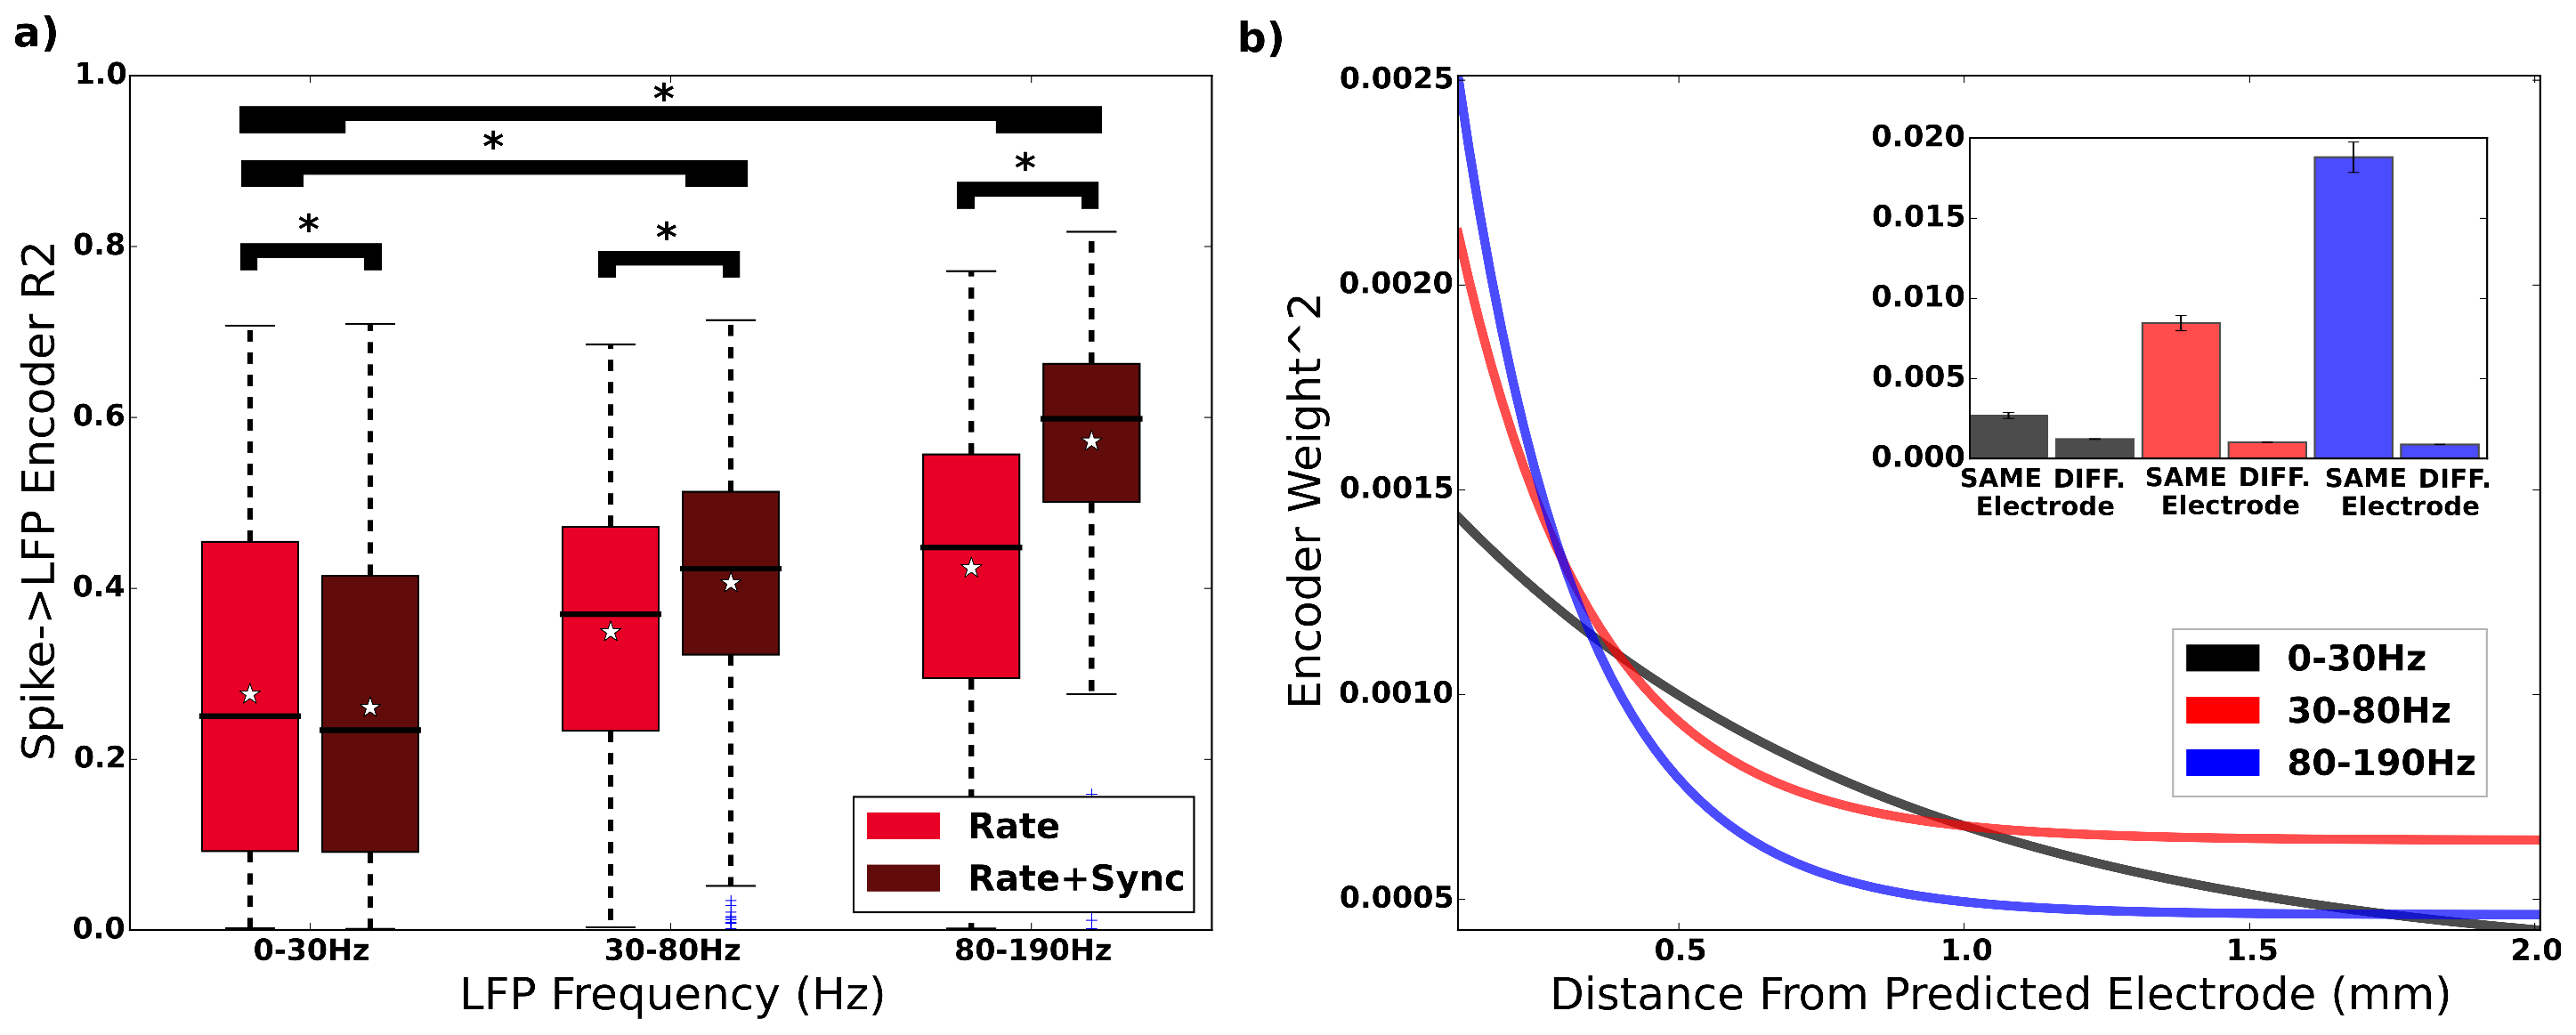
\includegraphics[scale=0.25]{figure8.eps}
\end{figure}


\section{Discussion}

In this work we have shown that Zebra finch syllables can be quantified by their acoustic features in a duration-independent fashion, that some of these acoustic features, mainly amplitude, spectral distribution statistics, pitch saliency, and temporal skew, can be used to predict both spike rate and LFP power. We showed that these features can be decoded from the spike rate vector of a population of neurons, and that the decoding performance grows as more neurons are utilized. We showed that the power spectrum of the LFP in the Zebra finch auditory system contains a significant amount of information about the acoustic features of vocalizations, and that regional differences exist in the type of information decoded.

    Training encoders enabled us to say what causally drove spike rate or LFP power on individual neurons or electrodes \cite{Weichwald2015}, while decoders enabled us to determine the nature of ensemble encoding by population activity (Figure 7). The acoustic features that drove neurons the most, such as maximum amplitude and spectral shape, were also acoustic features that were well decoded. We found that decoding from multi-electrode LFP power spectra gave performance on par with that of the population spike rate. This is an important finding for brain-machine interfaces, which could potentially forgo the computationally expensive step of spike identification and sorting for the cheaper alternative of simply computing the power spectra of the LFP.

    We found that decoding from population spike rate plus pairwise spike synchrony outperformed decoding from LFP power spectra or spike rate alone. This lends support to the idea that stimulus information can be carried by the pairwise activity of neurons, and is in potential conflict with findings by \cite{Ince2013}, who show that pairwise correlations do not contain additional stimulus information. Our approach differs from that research in that they broke their stimuli into categorical “tokens” prior to using an information theoretic approach to quantify the importance of correlations, which effectively determines whether pairwise correlations contain information about stimulus identity. In contrast, we used a decoding approach to show that acoustic features of stimuli were better decoded when pairwise terms were introduced. \cite{Ince2013} are effectively showing that pairwise correlations don’t contain information about stimulus identity. We are showing that pairwise correlations contain information about specific acoustic features. Because acoustic features can be similar between stimuli, a pairwise correlation code that carries information about acoustic features, will be similar for two acoustically similar but distinct stimuli, decreasing the ability of a decoder to discriminate stimulus identity but maintaining information about the relevant features.


The Zebra finch auditory system is not a homogenous structure. There is some evidence that it is anatomically layered in a way homologous to mammalian cortex \cite{Wang2010}. A detailed analysis of regional specificity by \cite{Meliza2012} showed that regions L2 and L1 were the least selective and tolerant, responding to most acoustic stimuli in a way that is not invariant to slight changes in acoustic features, while regions NCM and L3 were the most selective and tolerant. \cite{Elie2015a} analyzed the decoding performance of call type using the same dataset analyzed in this work, and found regional differences as well. They found that regions L3 and CM were the best at classifying Distance Calls and Field L were the best at classifying song. They also found that regions L3 and CMM was the most invariant (or tolerant) of variation in Distance calls. In our work, we found regions L2, L1, and CM were most effective for decoding maximum amplitude and mean spectral frequency, while region NCM was the least effective. We interpret this as showing NCM to be more invariant to amplitude and mean spectral frequency than other regions. We also found region L3 to less predicted by amplitude, which could contribute to its tolerance to acoustic perturbations in vocalizations found in other work.

    Finally, we demonstrated a concrete relationship between the local spike rate and spike synchrony, and LFP power that the population produces. If the LFP is comprised predominantly of synaptic currents, then we are showing that those synaptic currents are directly translated into the average spike rates of neurons, and enabled us to predict the LFP power from spike rate. We found that the addition of spike synchrony boosted our predictive power for the 30-80Hz and 80-190Hz frequency bands. The exponential curve fits shown in Figure 8b did not fit the data perfectly; there was much noise in the relationship between distance from predicted electrode and squared-weight. This noise could be due to differences in neuron density and electrical properties over space.


\section{Methods}

Electrophysiological methods and acoustic analyses are fully described in \cite{Elie2015a} and \cite{Elie2015b} respectively and are summarized here below. We then describe in detail the computational methods processing and representing local field potentials (LFPs), and the encoding and decoding analyses. All animal procedures were approved by the Animal Care and Use Committee of the University of California Berkeley, and were in accordance with the NIH guidelines regarding the care and use of animals for experimental procedures.

\subsection{Animals}

The animal subjects studied were adult and juvenile zebra finches (Taeniopygia guttata) from the colonies of the Theunissen and Bentley labs (University of California, Berkeley, USA) (Figure 1a). The electrophysiology experiments were performed on four male and two female adults from the Theunissen lab colony. The acoustic recordings described in the next subsection involved twenty-three birds (eight adult males, seven adult females, four female chicks, four male chicks). Six adults (three males, three females) were borrowed from the Bentley lab.
The electrophysiology subjects were housed in unisex cages and allowed to interact freely with their cagemates. All subjects were in the same room and were could interact visually acoustically. The acoustic recordings were performed on pair-bonded adults housed in groups of 2-3 pairs. Chicks were housed with their parents and siblings.

\subsection{Zebra Finch Vocalization Types}

Zebra finches communicate using a repertoire of vocalizations that are dependent on behavioral context. Following \cite{Zann1996}, acoustic signatures and behavioral contexts were used to classify vocalizations into nine different categories (Figure 1d). A detailed description of call categories can be found \cite{Elie2015a}. We provide here, a very succinct summary of that characterization for a subset of the calls analyzed here and used in the neurophysiological experiments.

Song is a multi-syllable vocalization emitted only by males. Songs are comprised of repeating motifs of syllables, and in the dataset, have a duration of 1424 +/- 983ms. Song in zebra finches are used in pair bonding and mating behavior. The repertoire contains monosyllabic affiliative calls used to maintain contact. Distance calls are loud, used when not in visual contact, and longer in duration (169 +/- 49ms) than Tet calls, emitted when in visual contact during hopping movements, with a duration of 81 +/- 16ms. Zebra finch also produce software calls used principally in the initial stages of pair bonding. Nest calls are soft monosyllabic vocalizations emitted by zebra finches looking for a nest or constructing a nest. With a duration of 95 +/- 75ms, they are similar to Tets.

Zebra finches emit two types of calls when they are acting out aggressively or being attacked. Wsst calls are noisy (broadband) and often long (503 +/- 499ms) calls emitted by a zebra finch when it is being aggressive. Distress calls are long (452 +/- 377ms), loud, and high-pitched vocalizations emitted by a zebra finch when escaping from an aggressive cage-mate. Both types of vocalizations can be mono or polysyllabic.

Two calls are emitted by juveniles only. Long tonal calls are the precursor to the adult distance calls; they are loud, long (durations of 184 +/- 63ms) and monosyllabic, emitted when the chick is separated from it’s siblings or parents. Begging calls are emitted when a juvenile zebra finch is begging for food from a parent, it is loud, long (duration of 382 +/- 289ms), and monosyllabic.


\subsection{Electrophysiology and Histology}

    Twenty-four hours before recording, the subject was deeply anaesthetized with isoflurane and injected topically with lidocaine in order to remove a patch of skin over the skull and cement a  head-holding fixture. On recording day, the subject was fasted for one hour, anaesthetized with urethane, head-fixed in a stereotaxic device, and two small rectangular openings were made over the auditory area of each hemisphere. An electrode array with two columns of eight tungsten electrodes was lowered into each hemisphere (Figure 1b,c). Electrodes were coated in DiI powder so that their path through the tissue could be analyzed post-experiment. The electrodes ran rostral-caudal lengthwise in eight rows, with two columns that ran medial-lateral.

    During the experiment, the subject was placed in a soundproof chamber and electrode arrays were independently lowered. Probe stimuli were used to determine visually whether the areas were auditory. Once a reliable site was found, a stimulus protocol was played over speakers within the chamber (described in next subsection). When the stimulus protocol was complete, the electrodes were lowered deeper by at least 100$\mu$m before playing the protocol again at the next site.
Once the recordings were finished, typically after 4-5 recording sites, the subject was killed with an overdose of isoflurane, the brain was removed and fixed with paraformaldehyde. Coronal slices of 20$\mu$m were made with a cryostat and Nissl stained. The slices were examined under a microscope and the DiI tracts were used to determine electrode penetration through anatomical regions. Six auditory areas were differentiated: three regions of field L (L1, L2, L3), caudomedial and caudolateral mesopallium (CMM and CML), and caudomedial nidopallium (NCM).


\subsection{Stimulus Protocol}

    The vocalizations of ten individuals (three adult females, three adult males, four chicks) were used in the stimulus protocol. The vocalizations of four of the individuals (one male adult, one female adult, one male chick, one female chick) were played at each recording site, and three of each vocalization type were randomly selected from the other birds to be played. Each vocalization was played on average 10 times, randomly interleaved with other vocalizations. The protocol lasted an average of one hour. Monosyllabic vocalizations such as Distance and Tet calls were played with 3-4 different renditions in series with inter-syllable intervals chosen to match what was observed naturally.


\subsection{Syllable Segmentation}

For this work we segmented all call types into syllables including Songs and Begging calls. The amplitude envelope of the series of call syllables was used for the segmentation. First the spectrogram was computed, and then the standard deviation of power across frequencies was computed at each time point to produce a time-varying amplitude envelope. Syllables began when the amplitude envelope exceeded a threshold value set to the 2nd percentile of the amplitude envelope distribution for all syllables. The syllable was marked as completed when the amplitude envelope subsequently dropped below this threshold. Syllables separated by 20ms or less were considered as one event.


\subsection{Acoustic Features}

    We used a classic bio-acoustical approach to estimate a complete set of acoustic features of each syllable, referred to as “Predefined Acoustical Features” described extensively in the Methods of \cite{Elie2015b} and summarized here. The 20 acoustic features fall into three different categories - temporal, spectral, and fundamental features.
    Temporal features were computed from the temporal envelope of the syllable. The temporal envelope was computed by rectifying the syllable’s raw sound pressure waveform and low-pass filtering with a cutoff frequency of 20 Hz. The temporal envelope was normalized by its sum, turning it into a probability distribution. The mean (Mean T), standard deviation ({\em Std T}), skew ({\em Skew T}), kurtosis ({\em Kurt T}), and entropy ({\em Ent T}) were computed and used as features. The peak amplitude of the syllable was computed as the peak of the non-normalized temporal envelope, and labeled as Max A.

Spectral features were computed from the spectral envelope, which is the power spectrum computed from the raw syllable sound pressure waveform. As was done for the temporal envelope, the spectral envelope was normalized by its sum, and the mean ({\em Mean S}), standard deviation ({\em Std S}), skew ({\em Skew S}), kurtosis ({\em Kurt S}) and entropy ({\em Ent S}) were computed. In addition, the 25th, 50th, and 75th percentile of the distribution were computed, and labeled as Q1, Q2, and Q3, respectively.

Time-varying fundamental features were computed from the spectrogram of the syllable and other properties. A feature was computed to quantify the degree of periodicity or pitch saliency of the syllable. To compute this feature, first the auto-correlation of the raw sound pressure waveform was computed. The peak in the auto-covariance at non-zero lag was found, and the saliency was then computed as the ratio between that peak value and the value of the auto-correlation at lag zero. The saliency feature was labeled as Saliency.

    The pitch for all time windows where the saliency was greater than 0.5 was computed by fitting the power spectrum at a time point with that of an idealized harmonic stack. Deviations from this idealized harmonic stack were used to quantify inharmonic properties, such as the presence of a second peak in the spectrum not explained by the stack. This ``double voice phenomenon'' was the result of the two independently driven vocal folds found in the syrinxes of songbirds \cite{Suthers1994}. Songs birds are capable of producing two independent voices although this is relatively rare in the zebra finch where the two folds are typically synchronized. The second fundamental frequency in this situations was computed as the acoustic feature {\em Pk 2}, and the acoustic feature {\em 2nd V} was defined as the percent of time a second voice was found. Other acoustic features describing the time-varying fundamental are the maximum, minimum, mean, and coefficient of variation in the fundamental frequency over time, labeled {\em Max F0}, {\em Min F0}, {\em Mean F0}, {\em CV F0}, respectively.


\subsection{LFP Power Spectrum Calculation}
    
    The local field potential was recorded with a sample rate of 381 Hz, limiting the maximum frequency of analysis to 190 Hz. The LFP on each electrode was z-scored across time for the duration of a stimulus protocol. The LFP was analyzed starting from the onset of a syllable, and the window of analysis was extended to 30ms following the syllable offset. Syllables of duration less than 40ms or more than 400ms were excluded from analysis.

    We will denote the z-scored LFP conditioned on a stimulus $s$, for trial $m$, electrode $k$ as $u_k ^m (t, s)$. We computed the LFP power spectrum from the Gaussian-windowed short-time Fourier Transform (STFT). The time points in the spectrogram were spaced by an increment of $\Delta \tau$ = 5ms. The window size was $W$=0.060. The frequency spacing was constant across stimuli due to the fixed window size, equal to $f$ = 9.78 Hz, and ranged from 0 to 190 Hz. The value of the STFT, centered at time  and frequency $f$ was computed as:

\begin{center}
$z_k ^m (\tau, f, s) = \sum_{t=1}^{T}\; exp(-\frac{(t-\tau)^2}{2 \sigma_W}) \; exp(i 2 \pi f t) \; u_k^m (t, s)$
\end{center}


where i=$\sqrt{-1}$, $T$ is the duration of the stimulus in number of time points at sample rate $f_s$ = 381 Hz, and W was chosen such that 95\% of the mass of the Gaussian was contained in the window:

\begin{center}
$\sigma_W = \frac{W}{6}$
\end{center}

From the complex-valued STFT, we averaged power across  windowed segments, of which there were $T_W = floor(\frac{T}{W})$, to get the power spectrum for electrode $k$, trial $m$, stimulus $s$:

\begin{center}
$x_k^m (f, s) = \frac{1}{T_W} \sum _{\tau = 1}^{T_W} \; | z_k^m (\tau, f, s) | ^2$
\end{center}

Once the power spectra were computed for each trial, they were averaged across trials to produce an average power spectrum for stimulus s. Finally, the power spectra were binned into three bins: 0-30Hz, 30-80Hz, 80-190Hz. Power within a band was the sum of values for $x_k^m (f, s)$ within that band’s frequencies.

\subsection{Population Spike Rate and Spike Synchrony}

    The spike rate for cell $i$, trial $m$, stimulus $s$, was computed as the number of spikes divided by the duration of the stimulus. Let $N_i^m (s)$ be the number of spikes that occur during stimulus $s$, trial $m$, for cell $i$. Then the spike rate is given as:

\begin{center}
$r_i^m (s) = \frac{N_i^m (s)}{duration \; of \; s}$
\end{center}

The spike rate for cell i was averaged across trials to produce an average spike rate $r_i (s)$, and the the population spike rate vector for stimulus s was defined as the vector of average spike rates for $Q$ cells recorded at a given site:

\begin{center}
$r(s) = [r_1(s) \;\; ... \;\; r_Q (s)]$
\end{center}

    To compute spike rate synchrony for stimulus $s$, trial $m$, between cells $i$ and $j$, we first binned the spike trains for $i$ and $j$ using a bin size of 3ms. Spike synchrony was computed as:

\begin{center}
$\gamma _{ij} ^m (s)=\frac{\# \; bins\; where\; i\; and \; j\; spiked}{\sqrt{N_i^m(s) N_j^m (s)}}$ 
\end{center}

Spike synchrony was then averaged across trials to produce an average synchrony $\gamma _{ij}(s)$.


\subsection{Encoder and Decoder Dataset Construction}

    We used an encoding approach to determine what acoustic features drove individual neural responses, and a decoding approach to determine how much information about acoustic features was contained in ensemble activity. We defined the vector $\textbf{y}(s)$ to be a collection of neural states, associated with stimulus $s$. $\textbf{y}(s)$ was comprised of one or more of the following neural states: the multi-electrode LFP power spectra, (``LFP PSD''), the population spike rate vector (``Spike Rate''), or the pairwise synchrony for all pairs of neurons (``Spike Sync''). We defined a vector $\textbf{x}$(s) to be a collection of acoustic features associated with stimulus $s$. The encoder attempts to predict a single scalar neural feature $y_i(s)$ from the vector of acoustic features $\textbf{x}(s)$. The decoder attempts to predict a single acoustic feature $x_j (s)$ from the neural feature vector $\textbf{y}(s)$.

The dataset was constructed from one run of a stimulus protocol on a recording site. Each stimulus protocol typically contained around 130 vocalizations randomly presented 10 times each. After segmentation and trial averaging, there were roughly $D$=600 samples. Each protocol contained vocalizations from eleven different birds - seven adults and four chicks. 


\subsection{Acoustic Feature Decoder Optimization and Cross Validation}

The decoder tries to predict a single acoustic feature $x_j (s)$ from a vector of neural responses $\textbf{y}(s)$. We define the matrix $Y$ to be of size $D$x$M$, where $D$ is the number of syllables in the dataset, and $M$ is the number of neural features for a given representation. We define the matrix $X$ to contain $D$ rows and 1 column, each row contains value of the acoustic feature $x_j(s)$ for a different syllable $s$. For the LFP PSD neural features, $M$=48 (16 electrodes x 3 frequency bands). For the Spike Rate neural features, there were typically 25-35 cells per site, so $M$ ranged from 25-35, while for the spike synchrony features, $M$ ranged from 300 to 595. The vector $\textbf{y}$ was always z-scored prior to fitting, as was each column of $X$.
    Regression finds optimal linear model weights w and scalar intercept b that minimize the sum of squares error between the model prediction and the actual data:

\begin{center}
$L(X, y, w) = \| (Xw + b) - y \| ^2$
\end{center}

Given the high dimensionality of some of our feature spaces, it was important to regularize values of $w$, so that we did not overfit the data. We utilized Ridge regression with scikits.learn to do this regularization. Ridge regression computes the optimal weight vector $w$ as:

\begin{center}
$\textbf{w} = (X^T X - \alpha I)^{-1} X^T \textbf{y}$
\end{center}

the value $\alpha$ is a user-defined hyperparameter, high values $\alpha$ of force weights towards zero.
The value of the hyperparameter $\alpha$ is found using a cross-validated approach. Our goal was to find a value for $\alpha$ that maximized generalization performance. We tested 50 values of $\alpha$, chosen from a logarithmically spaced set that ranged from $10^{-2}$ to $10^6$. For each candidate value of $\alpha$, we divided the data into a training and validation set 50 different times, and trained the model on the training set to find a set of weights $\textbf{w}$, evaluating the performance on the test set. The value of $\alpha$ that had the best average performance on the 50 test sets was chosen as the optimal $\alpha$. We trained a final model on the entire dataset using the optimal $\alpha$, to produce a final set of weights used for analysis.

Vocalizations within the same call category for the same bird can be highly correlated, and may produce very similar neural responses. This could artificially inflate the performance. To control for this, the validation set was comprised of the vocalizations of two randomly chosen adults and two randomly chosen juveniles from the 11 birds in the dataset. The validation set always had at least one example of each call type.

We used the R2 averaged across validation sets, the ``cross-validated R2'', as a performance measure for our data. The formula for R2 is given as:

\begin{center}
$R2 = \frac{L_{null}-L}{L_{null}}$
\end{center}

where $L_{null}$ is the sum of squares error for a model that only tries to predict $\textbf{y}$ with the intercept term $b$. It is well known that the R2 increases when the number of features $M$ increases, but this does not apply to the R2 computed on validation sets, which enabled us to compare model performance between models with different numbers of parameters.


\subsection{Ensemble Decoding Analysis}

We computed the decoder performance for each acoustic feature as a function of the number of electrodes. To do this, we combined data for each site across hemispheres, giving a total of 32 electrodes per recording site. For each site, a number of electrodes was selected ranging from 1, 4, 8, up to 32 in increments of 4. Once the number of electrodes was selected, up to fifty different combinations of that number of electrodes were selected from the site data. A decoder was trained on each combination, using cross validated Ridge regression decoder methods described in previous sections. The validation R2 was computed for each electrode combination, and the mean R2 across combinations was reported as the performance for that site given the number of electrodes specified.

\subsection{Spline Basis Representation of Acoustic Features}

We assumed that the relationship between acoustic features and neural activity was potentially nonlinear by transforming each acoustic feature into a cubic spline basis \cite{Friedman2009}. A scalar acoustic feature $x_j (s)$ was replaced by a five dimensional projection into the following basis:

\begin{center}
$b_j (s) = [x_j \;\; x_j^2 \;\; [x_j^3 - k_1]_+ \;\; [x_j^3 - k_2]_+ \;\; [x_j^3 - k_3]_+ ]$
\end{center}

Where the $[...]_+$ operator is rectification, values less than zero are set to zero. The values for $k_i$ are called the knots and were chosen as the 25th, 50th, and 75th percentile of the distribution of values for acoustic feature $j$.


\subsection{Encoder to Predict Spikes and LFP from Acoustic Features}

The encoder tried to predict a single scalar neural output, in the form of a spike rate or power at a given frequency band, from a set of acoustic features. Each acoustic feature was z-scored and then projected into a spline basis, as described above. The spline basis values were accumulated into a vector and used as the regressors in an optimization procedure described above for the decoder, but in addition a stagewise procedure was used to select the smallest predictive subset of acoustic features. To accomplish this, a baseline regression was run with the basis functions of maximum amplitude, mean spectral frequency, and saliency as regressors, and the cross-validation R2 was recorded on this baseline ``active set''. In the next step, the improvement in R2 was computed for the addition of each remaining acoustic feature. The acoustic feature that produced the largest performance increase was added to the active set, and the process was repeated until no acoustic features were left that improved encoder performance. The algorithm completed by recording the acoustic features in the active set and their incremental improvements to R2.


\subsection{Tuning Curves}

To compute a tuning curve for an acoustic feature, the weights of a trained encoder model that corresponded to that feature were dot multiplied by the spline basis representation of that feature, producing a value representing the contribution to neural response by that acoustic feature. To produce the points that comprised the tuning curve, a spline basis matrix was computed for 20 regularly spaced points across the acoustic feature range, and this 20x5 matrix multiplied the 5 weights corresponding to that acoustic feature, to produce 20 values of neural response contribution (spike rate, LFP power) on the interval.


\subsection{Predicting LFP Power from Population Spike Rate}

In addition to trying to predict neural features from acoustic features, we also build an encoder that attempted to predict LFP power for a given frequency and electrode from the population spike rate vector and spike synchrony features. The dataset construction was the same as described for the relationship between neural and acoustic features, but each row of the data matrix $X$ was comprised of the population spike rate vector for a given stimulus, or in addition, the spike synchrony between each pair of cells. Each element of the dependent variable vector y was comprised of the LFP power for a given frequency and electrode. A separate encoder was trained for each frequency/electrode combination. Once the encoders were trained, we fit exponential curves to the scatter data that mapped distance from predicted electrode to neuron squared-weight, for the encoder that predicted LFP power from the population spike rate. The form of the exponential function was:

\begin{center}
$f(x) = A \; exp(-\frac{x}{\lambda}) + B$
\end{center}

The function was fit using the curvefit routine of scipy, and we reported the space constant as $\lambda$ a measure of spatial extent.

